% ENSF 608 final team project report, EcoCollect, Group 9.
% Builds with XeTeX (tested with Tectonic). All asset paths are relative to this folder.
% Repository copy: the cover leaves out personal details because the repository is public.
\documentclass[11pt,letterpaper]{article}

\usepackage[T1]{fontenc}
\usepackage{lmodern}
\usepackage[margin=1in]{geometry}
\usepackage{microtype}
\usepackage{graphicx}
\usepackage{xcolor}
\usepackage{array}
\usepackage{booktabs}
\usepackage{longtable}
\usepackage{tabularx}
\usepackage{enumitem}
\usepackage{needspace}
\usepackage{listings}
\usepackage{fancyhdr}
\usepackage{url}
\usepackage[hidelinks,pdftitle={ENSF 608 Final Team Project Report: EcoCollect},pdfauthor={Group 9}]{hyperref}

% the diagrams are PDF 1.7
\ifdefined\pdfminorversion\pdfminorversion=7\fi
\ifdefined\XeTeXversion\AtBeginDocument{\special{pdf:minorversion 7}}\fi

\newcommand{\evidencecommit}{8c17502} % commit on main that the reported results come from

% identifiers such as pickup_request may break after an underscore or a dot
\def\UrlBreaks{\do\_\do\.\do\/}
\urlstyle{tt}

\newcolumntype{L}[1]{>{\raggedright\arraybackslash}p{#1}}
\newcolumntype{Y}{>{\raggedright\arraybackslash}X}

\lstset{basicstyle=\ttfamily\footnotesize, columns=fullflexible, keepspaces=true,
  frame=single, framerule=0.3pt, rulecolor=\color{black!35}, xleftmargin=4pt, xrightmargin=4pt,
  breaklines=true, showstringspaces=false, upquote=false, aboveskip=6pt, belowskip=6pt}

\setlist{itemsep=2pt, topsep=4pt, parsep=0pt}
\setlength{\parindent}{0pt}
\frenchspacing
\setlength{\parskip}{6pt}
\renewcommand{\arraystretch}{1.15}
\emergencystretch=2em
\setcounter{tocdepth}{2}

\pagestyle{fancy}
\fancyhf{}
\fancyhead[R]{\small ENSF 608 \textbar{} EcoCollect}
\fancyfoot[C]{\small\thepage}
\setlength{\headheight}{14pt}

\begin{document}

\hypersetup{pageanchor=false}
\begin{titlepage}
\centering
\vspace*{0.4in}
{\Large\bfseries UNIVERSITY OF CALGARY\par}
\vspace{0.25in}
{\large MEng: Software Engineering\par}
{\large ENSF 608 (Databases)\par}
\vspace{0.5in}
{\LARGE\bfseries Final Team Project Report: EcoCollect\par}
\vspace{0.12in}
{\large Group 9 \textbar{} Fall 2026\par}
\vspace{0.4in}
\textbf{GitHub Repository:} \url{https://github.com/dannydufau/ecocollect}\par
\vspace{0.2in}
\textbf{Professor:} Dr.\ Ronnie de Souza Santos, PhD\par
\vspace{0.5in}
\begin{tabular}{@{}cL{3.4in}@{}}
\toprule
\textbf{No.} & \textbf{Team member} \\
\midrule
1 & Krunaliben Patel \\
2 & Vedant Patel \\
3 & Saad Ahmad Malik \\
4 & Jasdeep Singh Malhotra \\
5 & Satyam Bhanot \\
6 & Danny Dufau \\
\bottomrule
\end{tabular}
\end{titlepage}
\hypersetup{pageanchor=true}

\enlargethispage{3\baselineskip}
{\setlength{\parskip}{0pt}\small\tableofcontents\par}
\clearpage

%----------------------------------------------------------------------
\section{Introduction}
\label{sec:introduction}

\subsection{Problem and System}
Taking old electronics to a recycling location can be difficult for Calgary residents who do not have a vehicle or who have limited mobility or time. Electronics can be recycled at several locations in the city~\cite{calgary}. EcoCollect is a web application that connects these residents with volunteers who can make the trip. A resident posts a pickup request with one-hour pickup windows. A volunteer accepts one window, collects the items and records their delivery to a recycling facility with a photo.

\subsection{Purpose and Scope of the Database}
PostgreSQL stores EcoCollect's operational records: accounts and roles, accepted terms, pickup requests and their history, assignments and deliveries, recycling facilities, EcoPoints awards and notifications. Two kinds of data are held elsewhere. Firebase Authentication handles sign-in and holds email addresses, and ImageKit stores the photo files. The database keeps each photo's file identifier and path.

The course model has 25 relations and 100 attributes in four schemas: \path{users} (6 tables), \path{requests} (9), \path{rewards} (3) and \path{notifications} (7). The application also uses tables for outgoing and processed events, idempotency keys and scheduled expiry jobs. These support communication between services and are outside the course model.

\subsection{Key Business Rules}
The conceptual model records 66 business rules, listed in Appendix~\ref{app:rules}. The following rules shape most of the design.
\begin{itemize}
  \item An account holds the Resident role, the Volunteer role or both, and its holder must be at least 18 at registration (BR1, BR6).
  \item A volunteer may save up to three Calgary postal codes for notifications (BR7, BR9).
  \item A request offers one to three distinct one-hour windows that start in the future and end within 30 days of its creation. It has at most one unfinished assignment at a time (BR20, BR32).
  \item Either party may cancel before collection is confirmed, but the resident only until the selected window ends. After that the resident confirms collection or reports a missed pickup (BR22).
  \item A missed request may be rescheduled once, as a new request linked to it (BR50).
  \item A delivery earns separate awards for the volunteer and the resident. A resident cancellation made less than 24 hours before the window starts earns the volunteer an award, unless the volunteer is also the resident (BR11). A volunteer award is $3 \times \textrm{quantity} + 4 \times \textrm{estimated weight in kg}$; a resident award is half of that (BR41).
\end{itemize}

\subsection{Continuity with the Project Proposal}
\label{sec:continuity}
The purpose of the system, its Calgary e-waste setting and its Sustainable Development Goal match our project proposal. We refined the preliminary entities while modelling and normalizing the data, and narrowed some of the proposed scope and behaviour. Table~\ref{tab:continuity} records the differences.

\begin{table}[!ht]
\centering\small
\caption{Differences between the project proposal and the final design}
\label{tab:continuity}
\begin{tabularx}{\linewidth}{@{}L{0.36\linewidth}Y@{}}
\toprule
Proposal & Final design \\
\midrule
Moderator and LoggedComplaint entities & Not included. Moderation and complaints are outside the final scope. \\
RequestItem entity & Each request holds one category, quantity and estimated weight. A submission with several categories creates one request for each, sharing one terms acceptance (BR43). \\
PostalCode entity & Postal codes are six-character values with a format check. \\
PickupRecord entity & Collection and missed-pickup facts are held in \path{assignment} and \path{status_change}. \\
DeliveryRecord with a drop-off location & \path{delivery} references a \path{recycling_facility} and an evidence photo. \\
User, ItemType, TermsAcceptanceRecord, Ecopoints, RequestStatusHistory & \path{account}, \path{item_category}, \path{terms_acceptance} with \path{terms_document}, the award relations and \path{status_change}. \\
Not proposed as entities & Facility acceptance, photos, preferred postal codes, push subscriptions, request events and notification sources have their own relations. \\
\addlinespace
A missed pickup reopens the request & \emph{Missed} is a final status. The resident may reschedule once (BR22, BR50). \\
Open requests expire after 30 days and may be renewed & An Open request expires when its last active window starts, which is within 30 days of creation. An expired request cannot be renewed (BR33). \\
Residents enter approximate weights & The system estimates weight from quantity and the category's standard weight (BR31). \\
Password hashes and email verification are stored & Firebase Authentication handles them. Email is not stored in the database (BR56). \\
Resident addresses include geolocation & An address is a street and a postal code. \\
\bottomrule
\end{tabularx}
\end{table}

%----------------------------------------------------------------------
\section{Sustainable Development Goal 12}
\label{sec:sdg}
EcoCollect addresses United Nations Sustainable Development Goal 12, Responsible Consumption and Production~\cite{sdg12}. Target 12.4 concerns the environmentally sound management of chemicals and all wastes throughout their life cycle. Target 12.5 is to substantially reduce waste generation through prevention, reduction, recycling and reuse. Our system contributes to a narrow part of these targets: helping household electronics reach a recycling facility. Table~\ref{tab:sdg} shows how the database supports that goal. Query identifiers refer to Section~\ref{sec:operations}.

\begin{table}[!ht]
\centering\small
\caption{How the database supports SDG 12}
\label{tab:sdg}
\begin{tabularx}{\linewidth}{@{}L{0.20\linewidth}L{0.27\linewidth}Yl@{}}
\toprule
Question & Stored data & Rules that keep it meaningful & Queries \\
\midrule
What is offered for recycling? & \path{item_category}; request quantity and estimated weight & Weight is calculated from the category standard and kept with the request (BR30, BR31). & O1, G1, G2 \\
Where can it go? & \path{recycling_facility}, \path{facility_accepts} & A delivery must use a facility that accepts the category (BR28, BR66). & J1 \\
What was delivered? & \path{delivery}, \path{assignment}, \path{photo} & One delivery per assignment, each with its own evidence photo (BR25, BR60). & A1, C2, L1 \\
What went uncollected? & \path{status_change} & Status history is appended, and Open requests expire (BR17, BR33). & G3 \\
Who took part? & \path{ecopoints_award} and two role relations & Each award is earned through one role (BR11, BR41). & C1 \\
\bottomrule
\end{tabularx}
\end{table}

In our sample data, A1 and C2 report two delivered requests with a total estimated weight of 5.60~kg: three phones (0.60~kg) and two laptops (5.00~kg). These figures show what the database can report. They are not a measurement of environmental impact. Weights are estimates rather than scale readings, a delivery photo records a handover but does not verify how the items were recycled, and the three seeded facilities are placeholders rather than real Calgary locations.

%----------------------------------------------------------------------
\section{Conceptual Database Model}
\label{sec:conceptual}
The conceptual model has 20 entities and 27 relationships. Figures~\ref{fig:er-accounts} to~\ref{fig:er-notifications} show all the relationships in three views that can be read on paper, and Table~\ref{tab:entities} lists the attributes of each entity. Figure~\ref{fig:er-overview} is the complete Entity-Relationship diagram with every attribute. It is stored as vector graphics, so it can be enlarged on screen without loss of detail. The editable source, \path{ER-Diagram.drawio}, is part of our submission.

In the relationship views, a label such as \texttt{0..N} states how many instances of the nearby entity can be linked to one instance of the entity at the other end. A minimum of 1 therefore means that participation by the entity at the \emph{other} end is mandatory. Double rectangles mark weak entities and double diamonds their identifying relationships.

\begin{figure}[!ht]
\centering
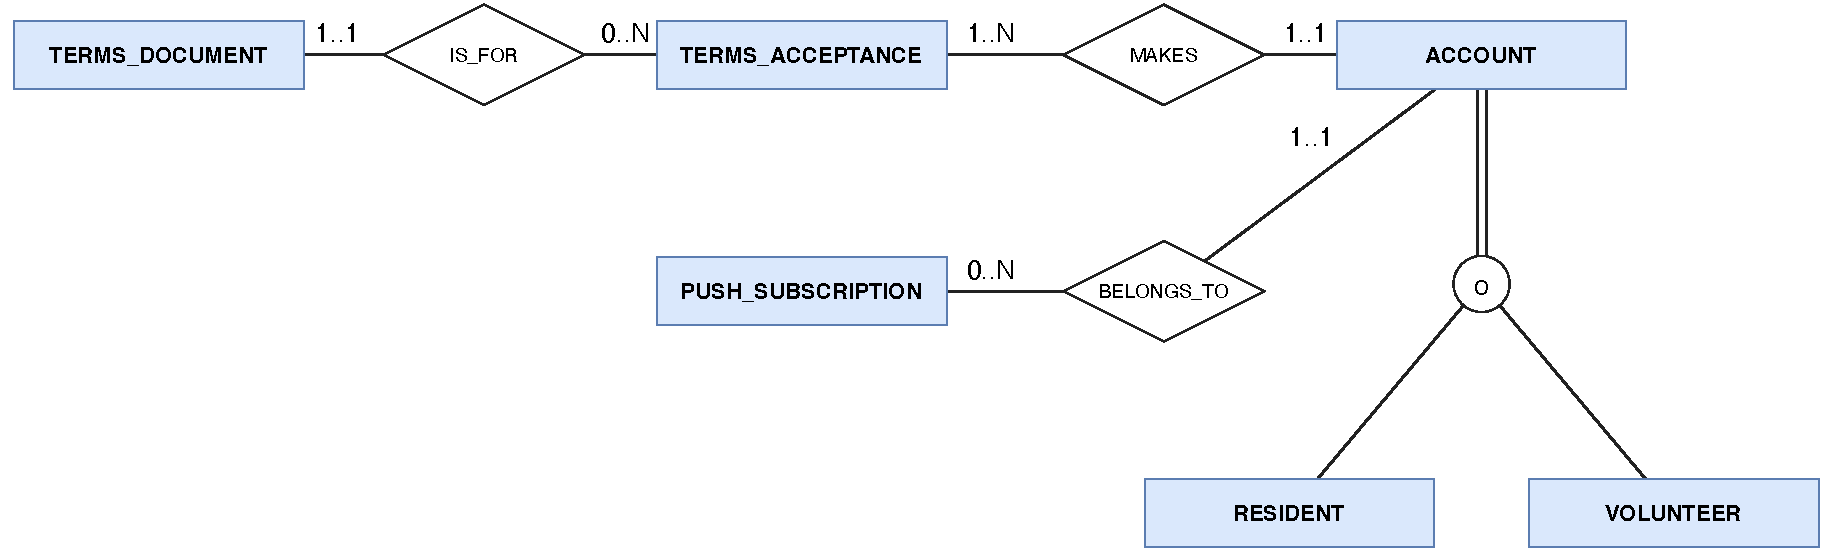
\includegraphics[width=\linewidth]{figures/er-accounts.pdf}
\caption{Relationship view 1: accounts, roles, terms and push subscriptions}
\label{fig:er-accounts}
\end{figure}

\begin{figure}[!ht]
\centering
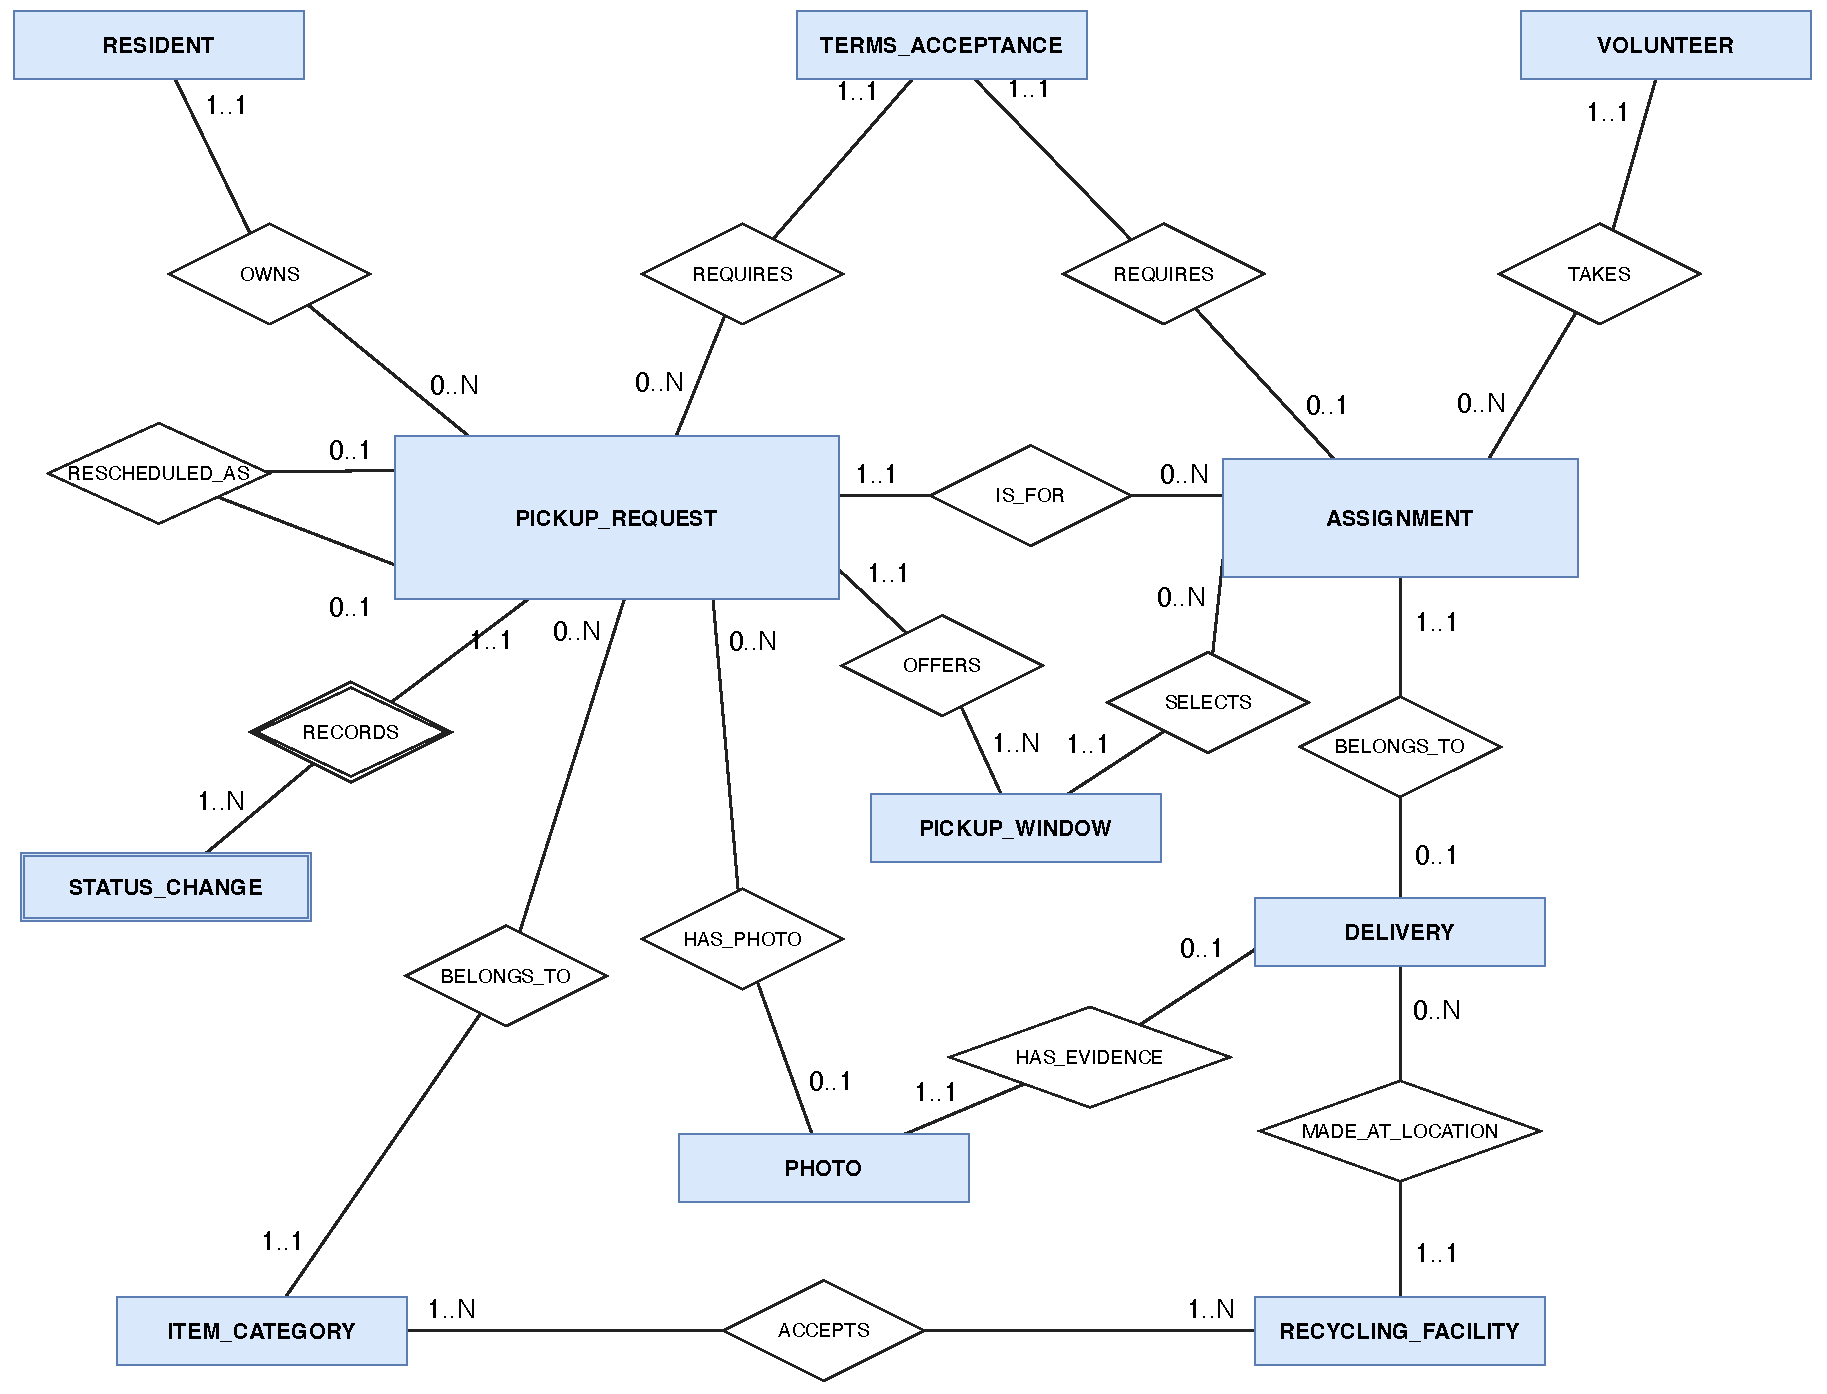
\includegraphics[width=\linewidth]{figures/er-requests.pdf}
\caption{Relationship view 2: requests, windows, assignments and deliveries}
\label{fig:er-requests}
\end{figure}

\begin{figure}[!ht]
\centering
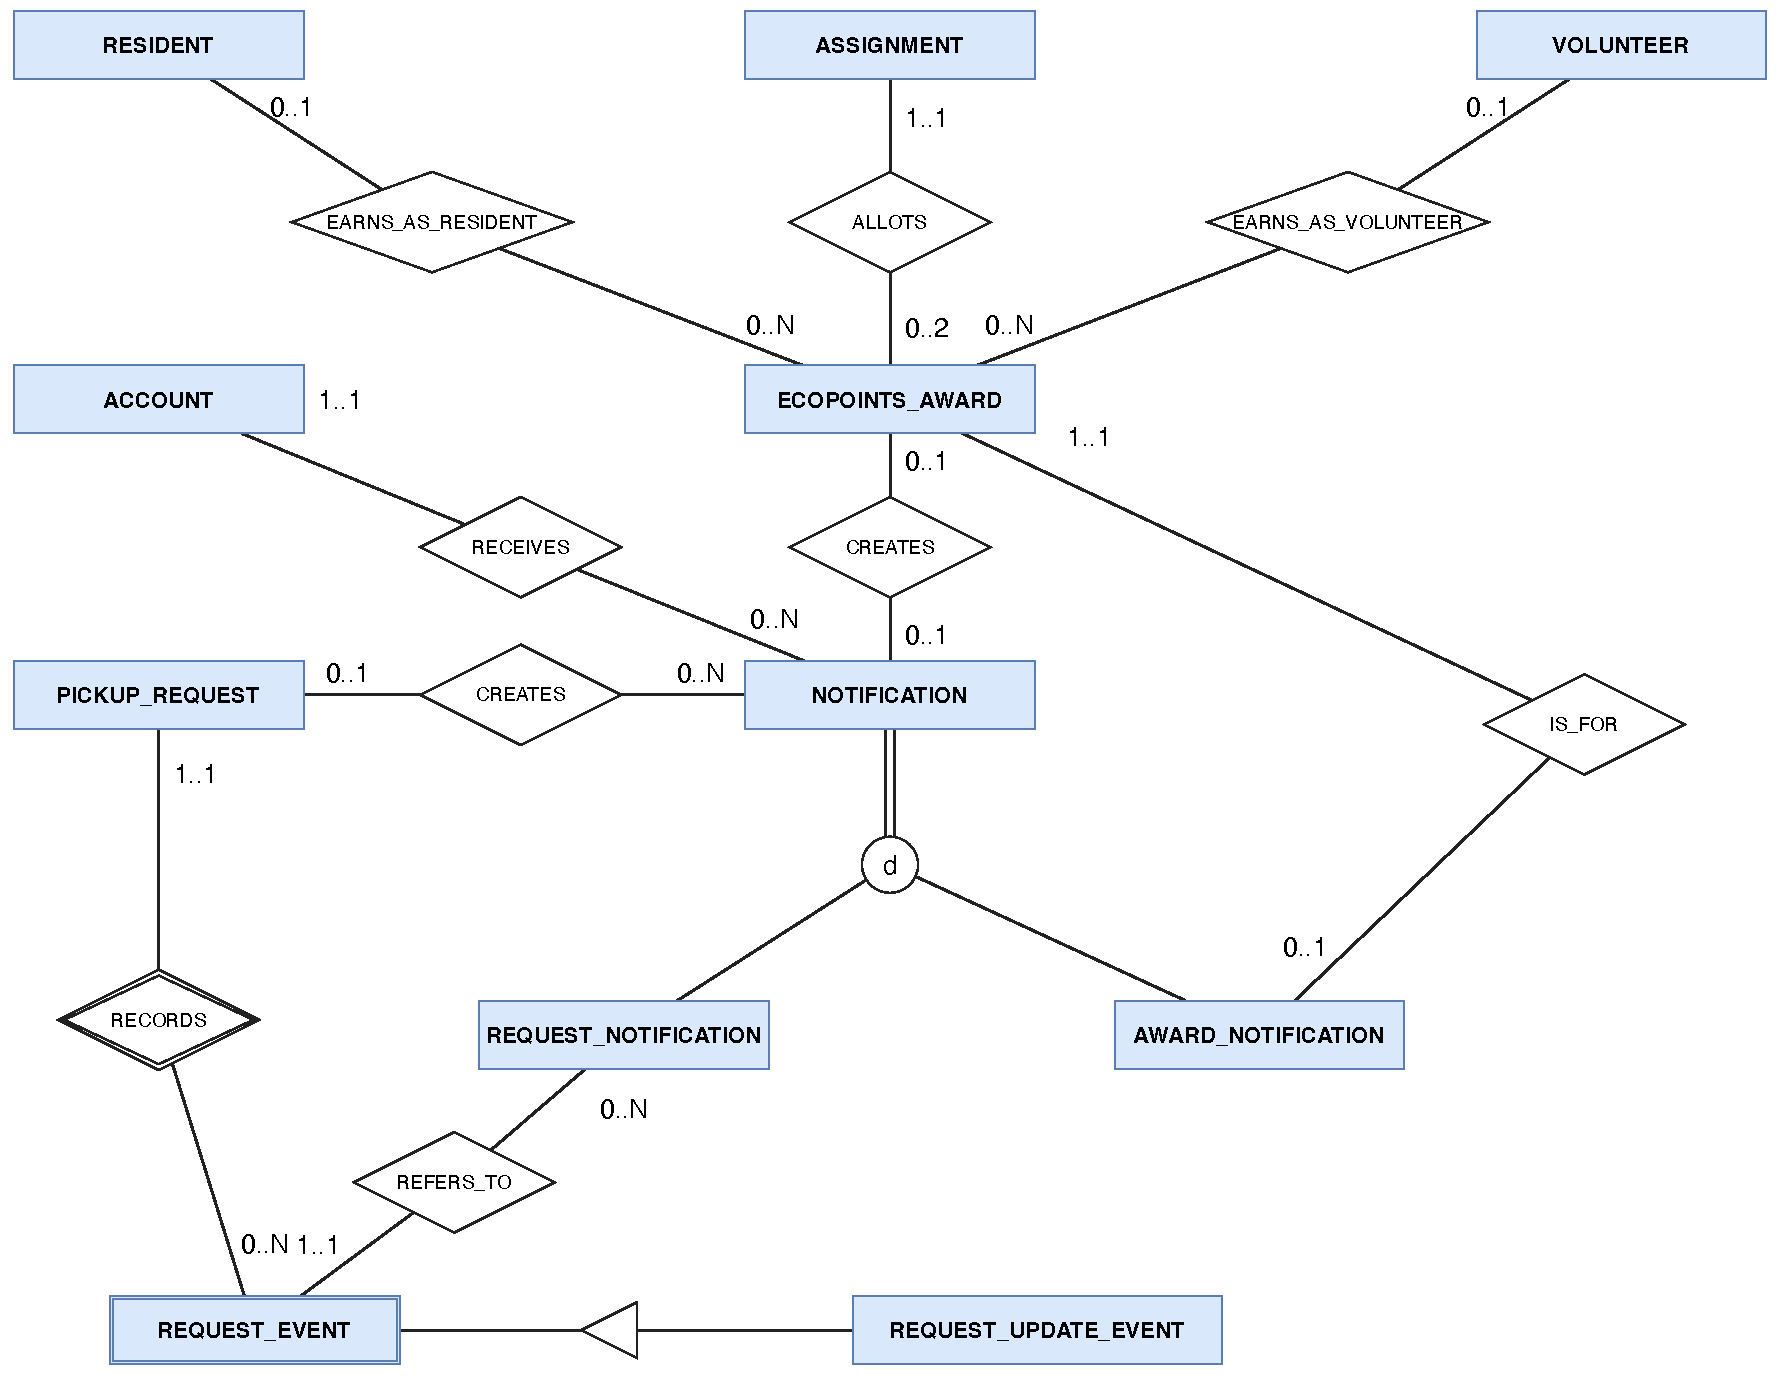
\includegraphics[width=\linewidth]{figures/er-notifications.pdf}
\caption{Relationship view 3: EcoPoints awards, request events and notifications}
\label{fig:er-notifications}
\end{figure}

\needspace{14\baselineskip}
\subsection{Entities and Attributes}
{\small
\begin{longtable}{@{}L{0.27\linewidth}L{0.17\linewidth}L{0.50\linewidth}@{}}
\caption{Entities, identifiers and attributes (M: multivalued; D: derived; composite parts in parentheses)}\label{tab:entities}\\
\toprule
Entity & Identifier & Other attributes \\
\midrule
\endfirsthead
\toprule
Entity & Identifier & Other attributes \\
\midrule
\endhead
\bottomrule
\endfoot
\path{ACCOUNT} & Account\_ID & Name (First\_Name, Last\_Name), Public\_Name, Date\_Of\_Birth, Created\_At, Deactivated\_At; D: Age, Combined\_Ecopoints \\
\path{RESIDENT} (subtype) & inherited & Address (Street, Postal\_Code) \\
\path{VOLUNTEER} (subtype) & inherited & M: Preferred\_Postal\_Code \\
\path{PUSH_SUBSCRIPTION} & Endpoint & P256dh, Auth, Expiration\_Time, User\_Agent, Updated\_At \\
\path{TERMS_DOCUMENT} & ID & Content, Published\_At \\
\path{TERMS_ACCEPTANCE} & ID & Accepted\_At, Type \\
\path{ITEM_CATEGORY} & ID & Name, Waste\_Type, Standard\_Weight\_Kg \\
\path{PHOTO} & File\_ID & File\_Path \\
\path{PICKUP_REQUEST} & ID & Quantity, Estimated\_Weight\_Kg, Created\_At, Request\_Seq, Notes, Pickup\_Address (Street, Postal\_Code); D: Status, Expires\_At, Deliverable\_Facilities \\
\path{PICKUP_WINDOW} & ID & Pickup\_Date, Start\_Hour, Is\_Active \\
\path{STATUS_CHANGE} (weak) & owner request and Changed\_At & Status, Reason \\
\path{ASSIGNMENT} & ID & Accepted\_At, Collected\_At, Ended\_At, End\_Reason; D: Status \\
\path{RECYCLING_FACILITY} & ID & Name, Address (Street, Postal\_Code), Special\_Instructions \\
\path{DELIVERY} & ID & D: Delivered\_At \\
\path{ECOPOINTS_AWARD} & ID & Points, Formula; D: Awarded\_At, Type \\
\path{NOTIFICATION} (supertype) & ID & Type, Created\_At, Pushed\_At, Is\_Read, Is\_Expired; D: Title, Body \\
\path{REQUEST_NOTIFICATION} (subtype) & inherited & D: Metadata \\
\path{AWARD_NOTIFICATION} (subtype) & inherited & none \\
\path{REQUEST_EVENT} (weak) & owner request and Request\_Seq & Transition\_ID \\
\path{REQUEST_UPDATE_EVENT} (subtype) & inherited & Reason; M: Changed\_Field \\
\end{longtable}
}

\subsection{Key Modelling Decisions}
\textbf{Roles as an overlapping, total specialization.} \path{ACCOUNT} specializes into \path{RESIDENT} and \path{VOLUNTEER}. Every account has at least one role and may have both, so a person who offers and collects items needs only one account (BR1).

\textbf{Notification sources as a disjoint, total specialization.} A notification is either a \path{REQUEST_NOTIFICATION} or an \path{AWARD_NOTIFICATION}, never both (BR62). The two subtypes derive their recipient and content in different ways.

\textbf{Two weak entities.} \path{STATUS_CHANGE} is identified by its request together with Changed\_At, and keeps the request's lifecycle as appended history (BR17, BR18). \path{REQUEST_EVENT} is identified by its request together with Request\_Seq (BR63). It records an event that the notification service has received.

\textbf{Events separated from notifications.} One event can notify several accounts, so its facts are stored once in \path{REQUEST_EVENT} and referenced by notifications. Only edit and reopening events have a reason, which the partial specialization \path{REQUEST_UPDATE_EVENT} holds with the multivalued Changed\_Field (BR64).

\textbf{Assignments kept as history.} A request can have several assignments over time, for example after a volunteer cancels. Each selects one offered window, and replaced windows remain as inactive records (BR20, BR36).

\textbf{Derived values.} Values that follow from other facts, such as request status, expiry time, delivery time and point totals, are marked as derived and are not stored.

% turned sideways on its own float page, so the text before it is not cut short
\begin{figure}[p]
\centering
\rotatebox{90}{\begin{minipage}{0.97\textheight}
\centering
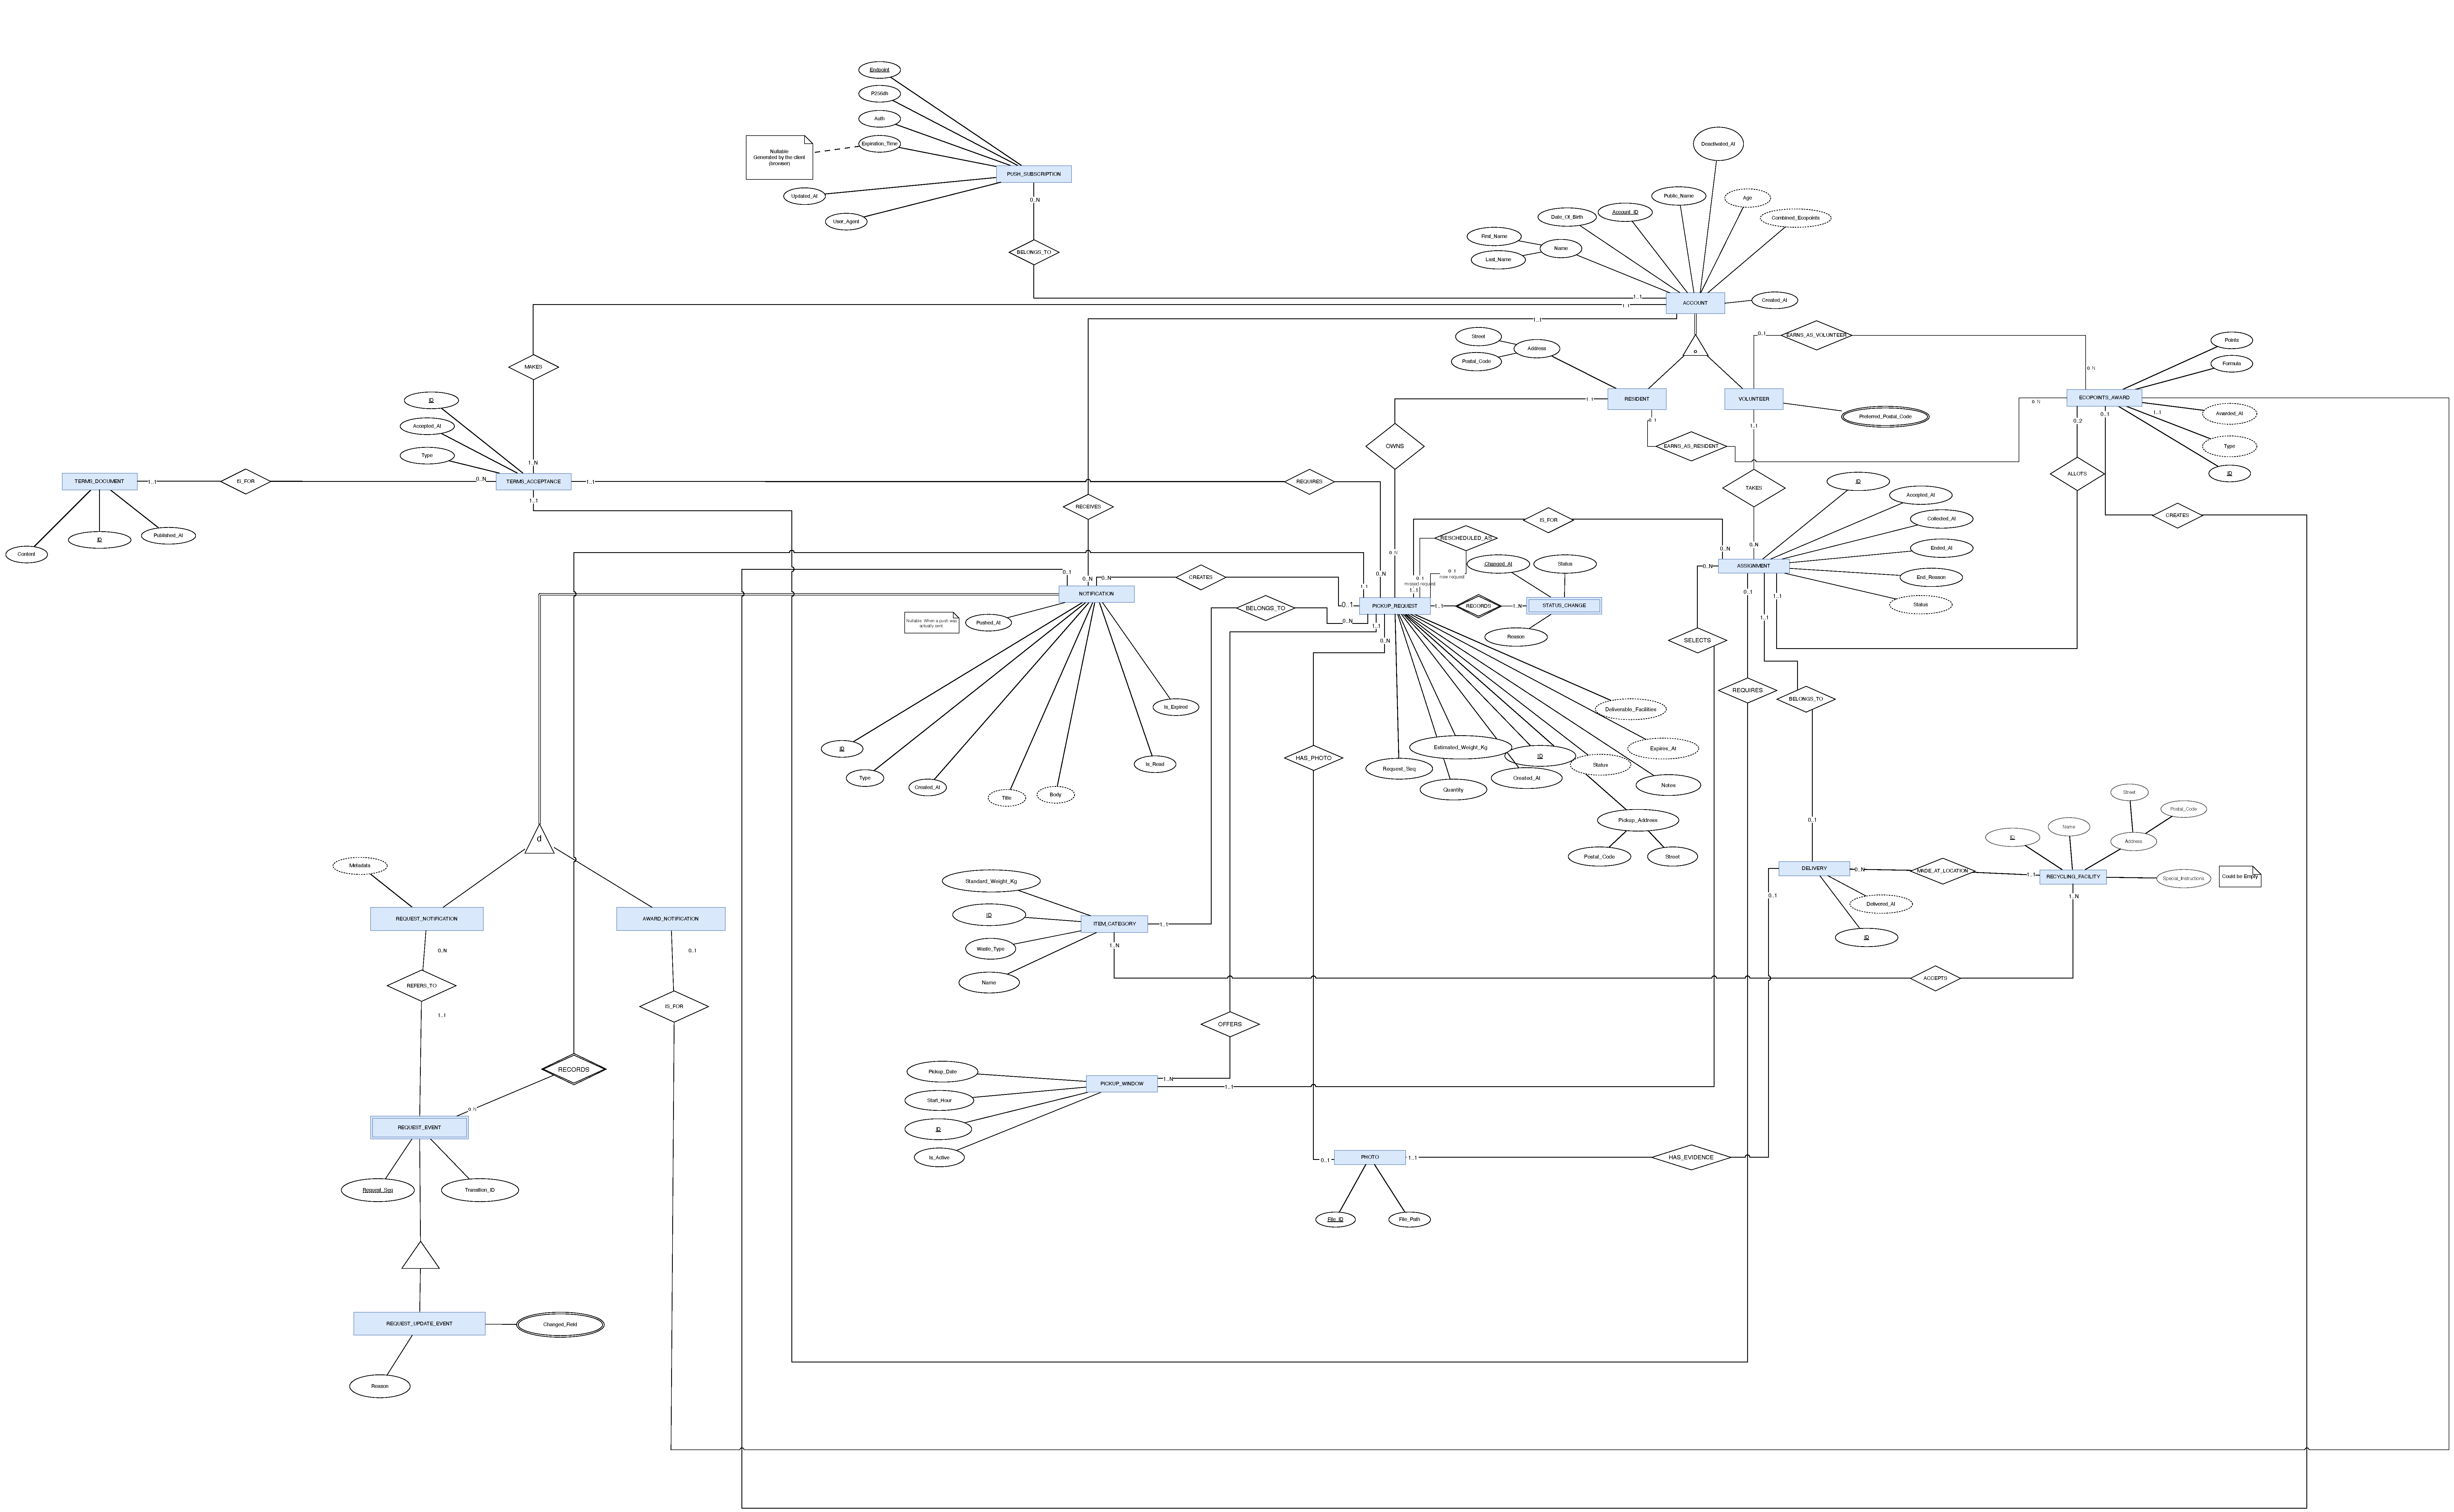
\includegraphics[width=\linewidth,height=0.9\linewidth,keepaspectratio]{figures/er-overview.pdf}
\caption{Complete conceptual ER diagram with entities and attributes. The note listing the business rules is reproduced in Appendix~\ref{app:rules}.}
\label{fig:er-overview}
\end{minipage}}
\end{figure}

%----------------------------------------------------------------------
\section{Logical Database Model}
\label{sec:logical}
The logical model maps the conceptual model to 25 relations with 25 primary keys and 30 foreign keys. Table~\ref{tab:mapping} gives the mapping rules, followed by the complete relational schema and its diagrams.

\subsection{Conceptual-to-Relational Mapping}
{\small
\begin{longtable}{@{}L{0.30\linewidth}L{0.66\linewidth}@{}}
\caption{Mapping from conceptual constructs to relations}\label{tab:mapping}\\
\toprule
Conceptual construct & Relational representation \\
\midrule
\endfirsthead
\toprule
Conceptual construct & Relational representation \\
\midrule
\endhead
\bottomrule
\endfoot
Strong entities & One relation each, with the identifier as primary key. \\
Account specialization & \path{account} holds shared facts. \path{resident} and \path{volunteer} use \path{account_id} as primary key and foreign key. \\
Composite attributes & Stored as separate columns, for example \path{pickup_street} and \path{pickup_postal_code}. \\
Multivalued attributes & \path{volunteer_preferred_postal_code} and \path{request_changed_field}, each with one value per row. \\
Weak entities & \path{status_change} uses (\path{pickup_request_id}, \path{changed_at}); \path{request_event} uses (\path{pickup_request_id}, \path{request_seq}). \\
One-to-many relationships & A foreign key on the ``many'' side, for example the category and window references. \\
Optional and one-to-one links & A delivery references its assignment through a unique foreign key. The evidence photo is also unique. A request's item photo is a nullable foreign key. \\
Rescheduling & Nullable, unique self-reference \path{rescheduled_from_request_id}. \\
Facility accepts category & Associative relation \path{facility_accepts} with a composite primary key. \\
Request owner and assignment volunteer & Reached through the required terms acceptance of the request or assignment. An assignment reaches its request through its window. \\
Award roles & \path{ecopoints_award} with role relations \path{resident_award} and \path{volunteer_award}. The recipient is reached through the assignment. \\
Relationships implied by other links & No column of their own. An assignment's request comes from \path{SELECTS}; the \path{EARNS_AS} links come from the award role and its assignment; both \path{CREATES} links to \path{NOTIFICATION} come from the notification's source. \path{RECEIVES} is stored as \path{account_id} for request notifications and derived through the award for award notifications. \\
Notification specialization & \path{notification} with \path{request_notification} or \path{award_notification}. An award notification reaches its recipient through the award. \\
Update-event specialization & \path{request_update_event} shares the composite key of \path{request_event}. \\
Derived attributes & Not stored. Queries and services compute them from the source facts. \\
\end{longtable}
}

\subsection{Relational Schema}
\label{sec:schema}
In the schema below, \underline{underlined} columns form the primary key, an asterisk marks a foreign key, and a question mark marks a nullable column. Each foreign key references the relation shown after the arrow.

{\small
\begin{longtable}{@{}L{0.97\linewidth}@{}}
\caption{Complete relational schema}\label{tab:schema}\\
\toprule
\endfirsthead
\toprule
\endhead
\bottomrule
\endfoot
\multicolumn{1}{@{}l}{\textbf{users}} \\
\path{account}(\underline{account\_id}, first\_name, last\_name, public\_name, date\_of\_birth, created\_at, deactivated\_at?) \\
\path{resident}(\underline{account\_id}*$\rightarrow$account, street, postal\_code) \\
\path{volunteer}(\underline{account\_id}*$\rightarrow$account) \\
\path{volunteer_preferred_postal_code}(\underline{account\_id}*$\rightarrow$volunteer, \underline{postal\_code}) \\
\path{terms_document}(\underline{terms\_document\_id}, content, published\_at) \\
\path{terms_acceptance}(\underline{terms\_acceptance\_id}, terms\_document\_id*$\rightarrow$terms\_document, account\_id*$\rightarrow$account, accepted\_at, type) \\
\addlinespace
\multicolumn{1}{@{}l}{\textbf{requests}} \\
\path{item_category}(\underline{category\_id}, name, waste\_type, standard\_weight\_kg) \\
\path{photo}(\underline{file\_id}, file\_path) \\
\path{pickup_request}(\underline{pickup\_request\_id}, category\_id*$\rightarrow$item\_category, terms\_acceptance\_id*$\rightarrow$terms\_acceptance, quantity, estimated\_weight\_kg, created\_at, request\_seq, pickup\_street, pickup\_postal\_code, notes?, file\_id?*$\rightarrow$photo, rescheduled\_from\_request\_id?*$\rightarrow$pickup\_request [unique]) \\
\path{pickup_window}(\underline{pickup\_window\_id}, pickup\_request\_id*$\rightarrow$pickup\_request, pickup\_date, start\_hour, is\_active) \\
\path{status_change}(\underline{pickup\_request\_id}*$\rightarrow$pickup\_request, \underline{changed\_at}, status, reason?) \\
\path{assignment}(\underline{assignment\_id}, pickup\_window\_id*$\rightarrow$pickup\_window, terms\_acceptance\_id*$\rightarrow$terms\_acceptance, accepted\_at, collected\_at?, ended\_at?, end\_reason?) \\
\path{recycling_facility}(\underline{facility\_id}, name, street, postal\_code, special\_instructions?) \\
\path{facility_accepts}(\underline{facility\_id}*$\rightarrow$recycling\_facility, \underline{category\_id}*$\rightarrow$item\_category) \\
\path{delivery}(\underline{delivery\_id}, assignment\_id*$\rightarrow$assignment [unique], facility\_id*$\rightarrow$recycling\_facility, file\_id*$\rightarrow$photo [unique]) \\
\addlinespace
\multicolumn{1}{@{}l}{\textbf{rewards}} \\
\path{ecopoints_award}(\underline{ecopoints\_award\_id}, assignment\_id*$\rightarrow$assignment, points, formula) \\
\path{resident_award}(\underline{ecopoints\_award\_id}*$\rightarrow$ecopoints\_award) \\
\path{volunteer_award}(\underline{ecopoints\_award\_id}*$\rightarrow$ecopoints\_award) \\
\addlinespace
\multicolumn{1}{@{}l}{\textbf{notifications}} \\
\path{push_subscription}(\underline{endpoint}, account\_id*$\rightarrow$account, p256dh, auth, expiration\_time?, user\_agent?, updated\_at) \\
\path{notification}(\underline{notification\_id}, type, created\_at, pushed\_at?, is\_read, is\_expired) \\
\path{request_event}(\underline{pickup\_request\_id}*$\rightarrow$pickup\_request, \underline{request\_seq}, transition\_id) \\
\path{request_update_event}(\underline{pickup\_request\_id, request\_seq}*$\rightarrow$request\_event, reason) \\
\path{request_changed_field}(\underline{pickup\_request\_id, request\_seq}*$\rightarrow$request\_update\_event, \underline{field\_name}) \\
\path{request_notification}(\underline{notification\_id}*$\rightarrow$notification, account\_id*$\rightarrow$account, (pickup\_request\_id, request\_seq)*$\rightarrow$request\_event) \\
\path{award_notification}(\underline{notification\_id}*$\rightarrow$notification, ecopoints\_award\_id*$\rightarrow$ecopoints\_award [unique]) \\
\end{longtable}
}

\subsection{Keys, Nullability and Domains}
Three further columns are candidate keys because each is required and unique: \path{assignment_id} and \path{file_id} in \path{delivery}, and \path{ecopoints_award_id} in \path{award_notification}. The nullable unique column \path{rescheduled_from_request_id} is not a candidate key for the whole relation. Only 12 columns accept nulls, shown with a question mark in Table~\ref{tab:schema}. Closed sets of values are used for request status (7 values), assignment end reason (4), acceptance type (4), update reason (2), changed field (5) and notification type (20). Column types and checks are given in Appendix~\ref{app:dictionary}.

\subsection{Relational Diagrams}
Figures~\ref{fig:rel-users} to~\ref{fig:rel-rewards} show the primary and foreign keys by area. Each arrow runs from the referencing relation to the referenced relation, and a composite foreign key is drawn once, from its first column. Dashed boxes stand for relations defined in another figure. Underlining marks primary-key columns, and a question mark marks nullable columns.

\begin{figure}[!ht]
\centering
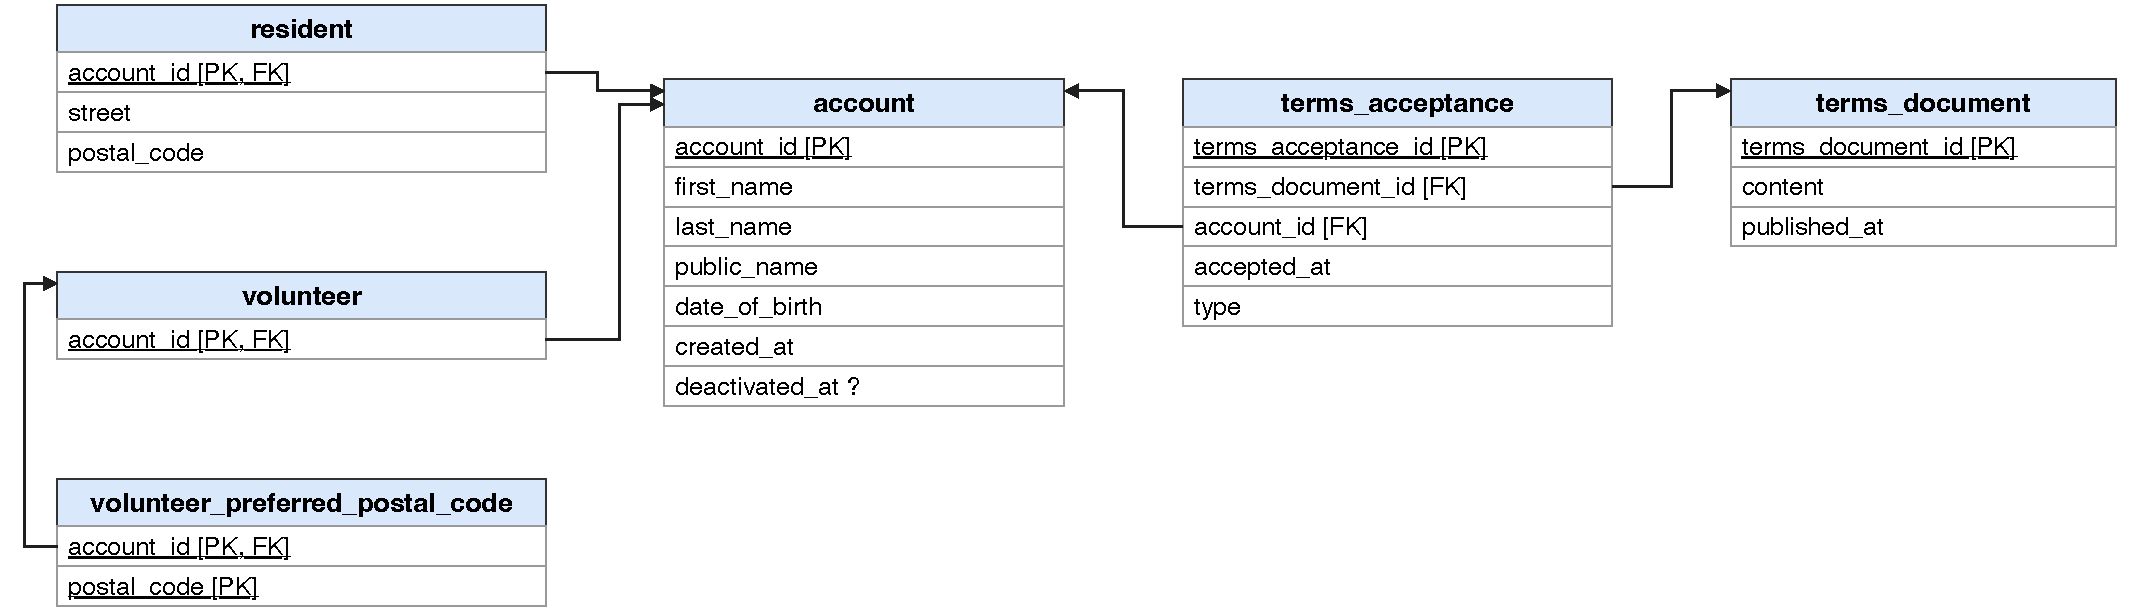
\includegraphics[width=\linewidth]{figures/rel-users.pdf}
\caption{Relational diagram: \texttt{users} schema}
\label{fig:rel-users}
\end{figure}

\begin{figure}[!ht]
\centering
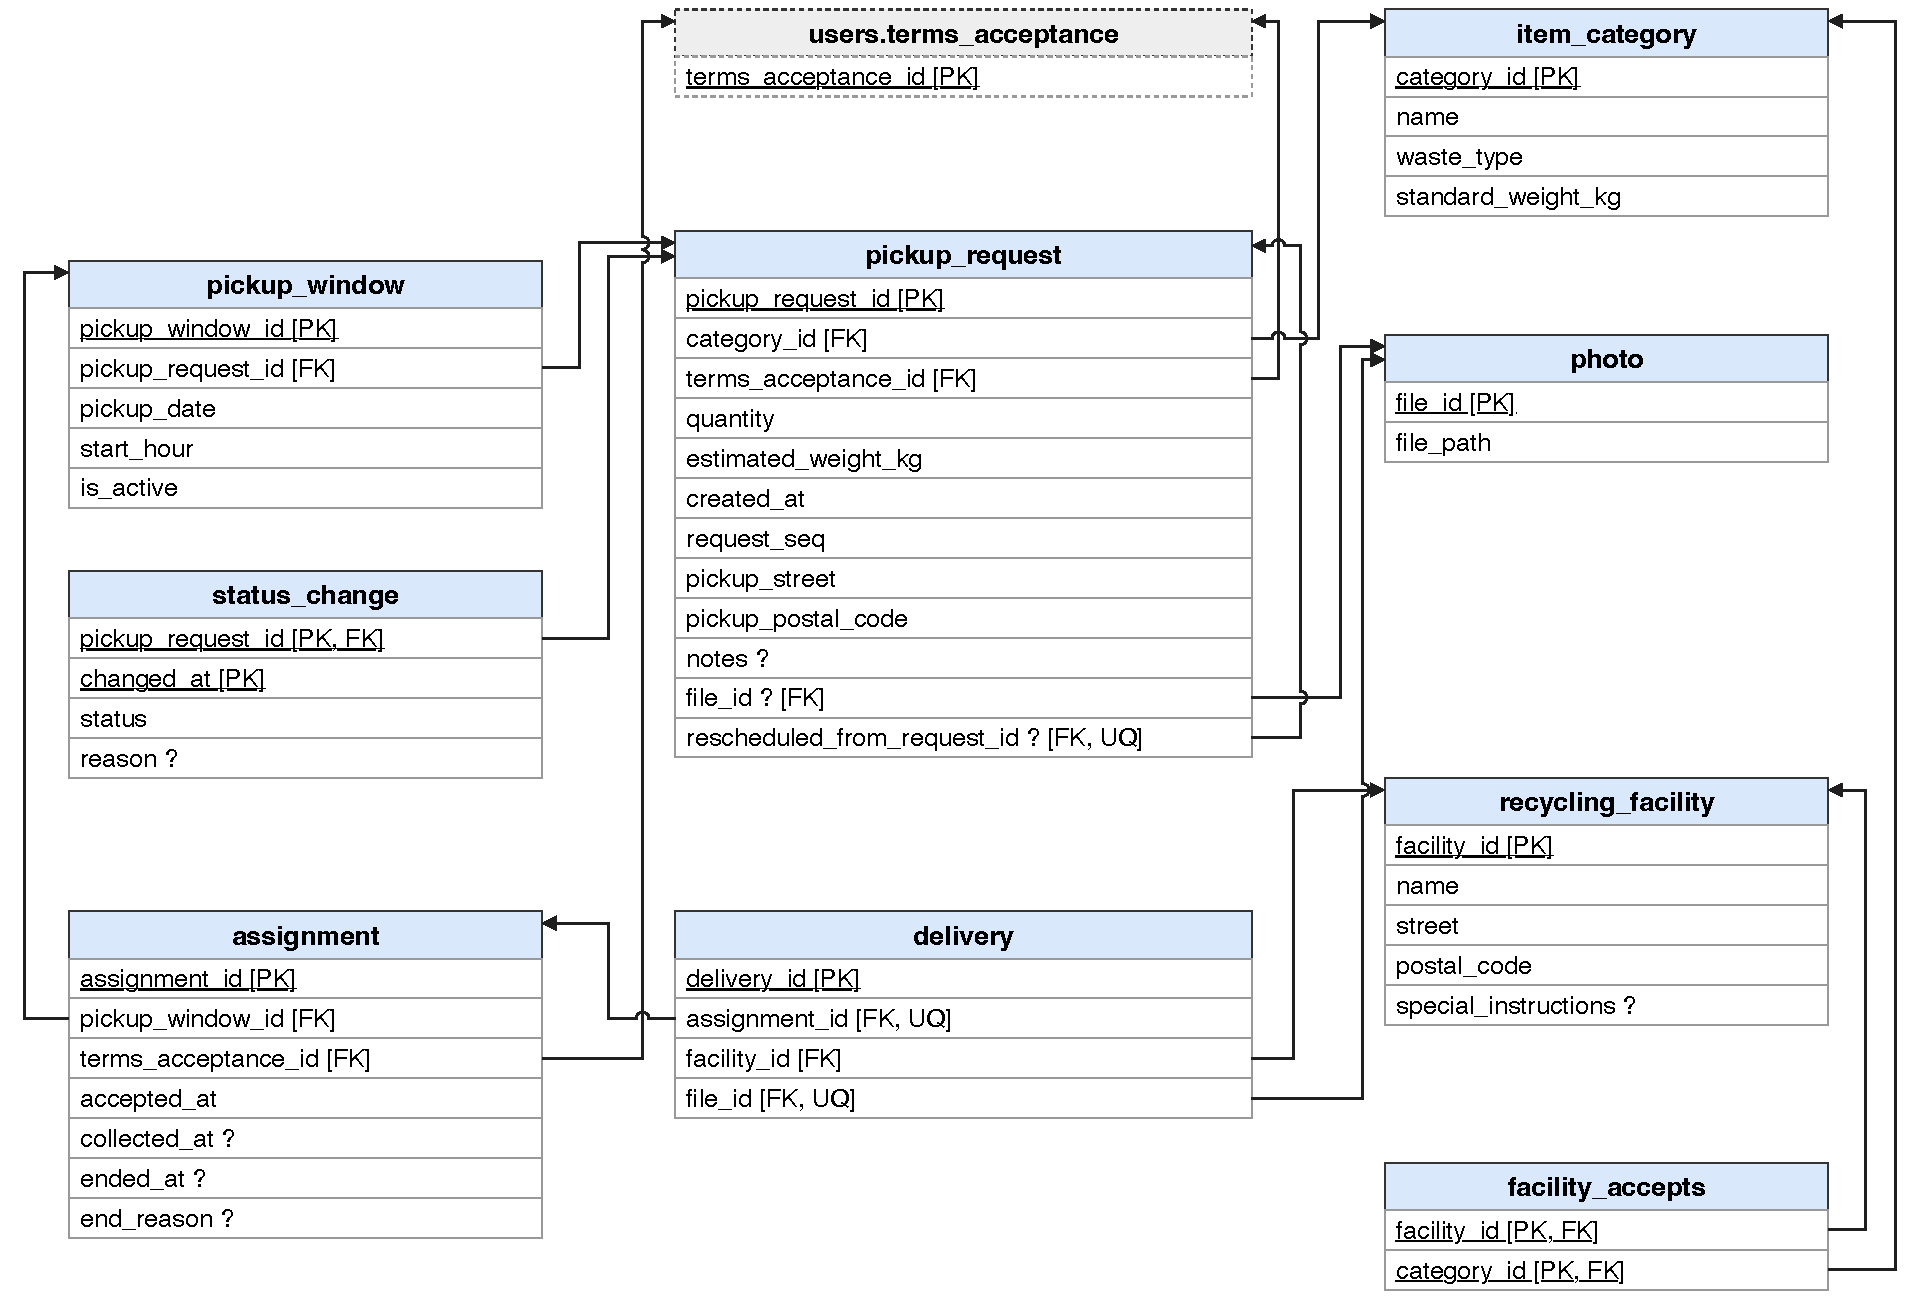
\includegraphics[width=\linewidth]{figures/rel-requests.pdf}
\caption{Relational diagram: \texttt{requests} schema}
\label{fig:rel-requests}
\end{figure}

\begin{figure}[!ht]
\centering
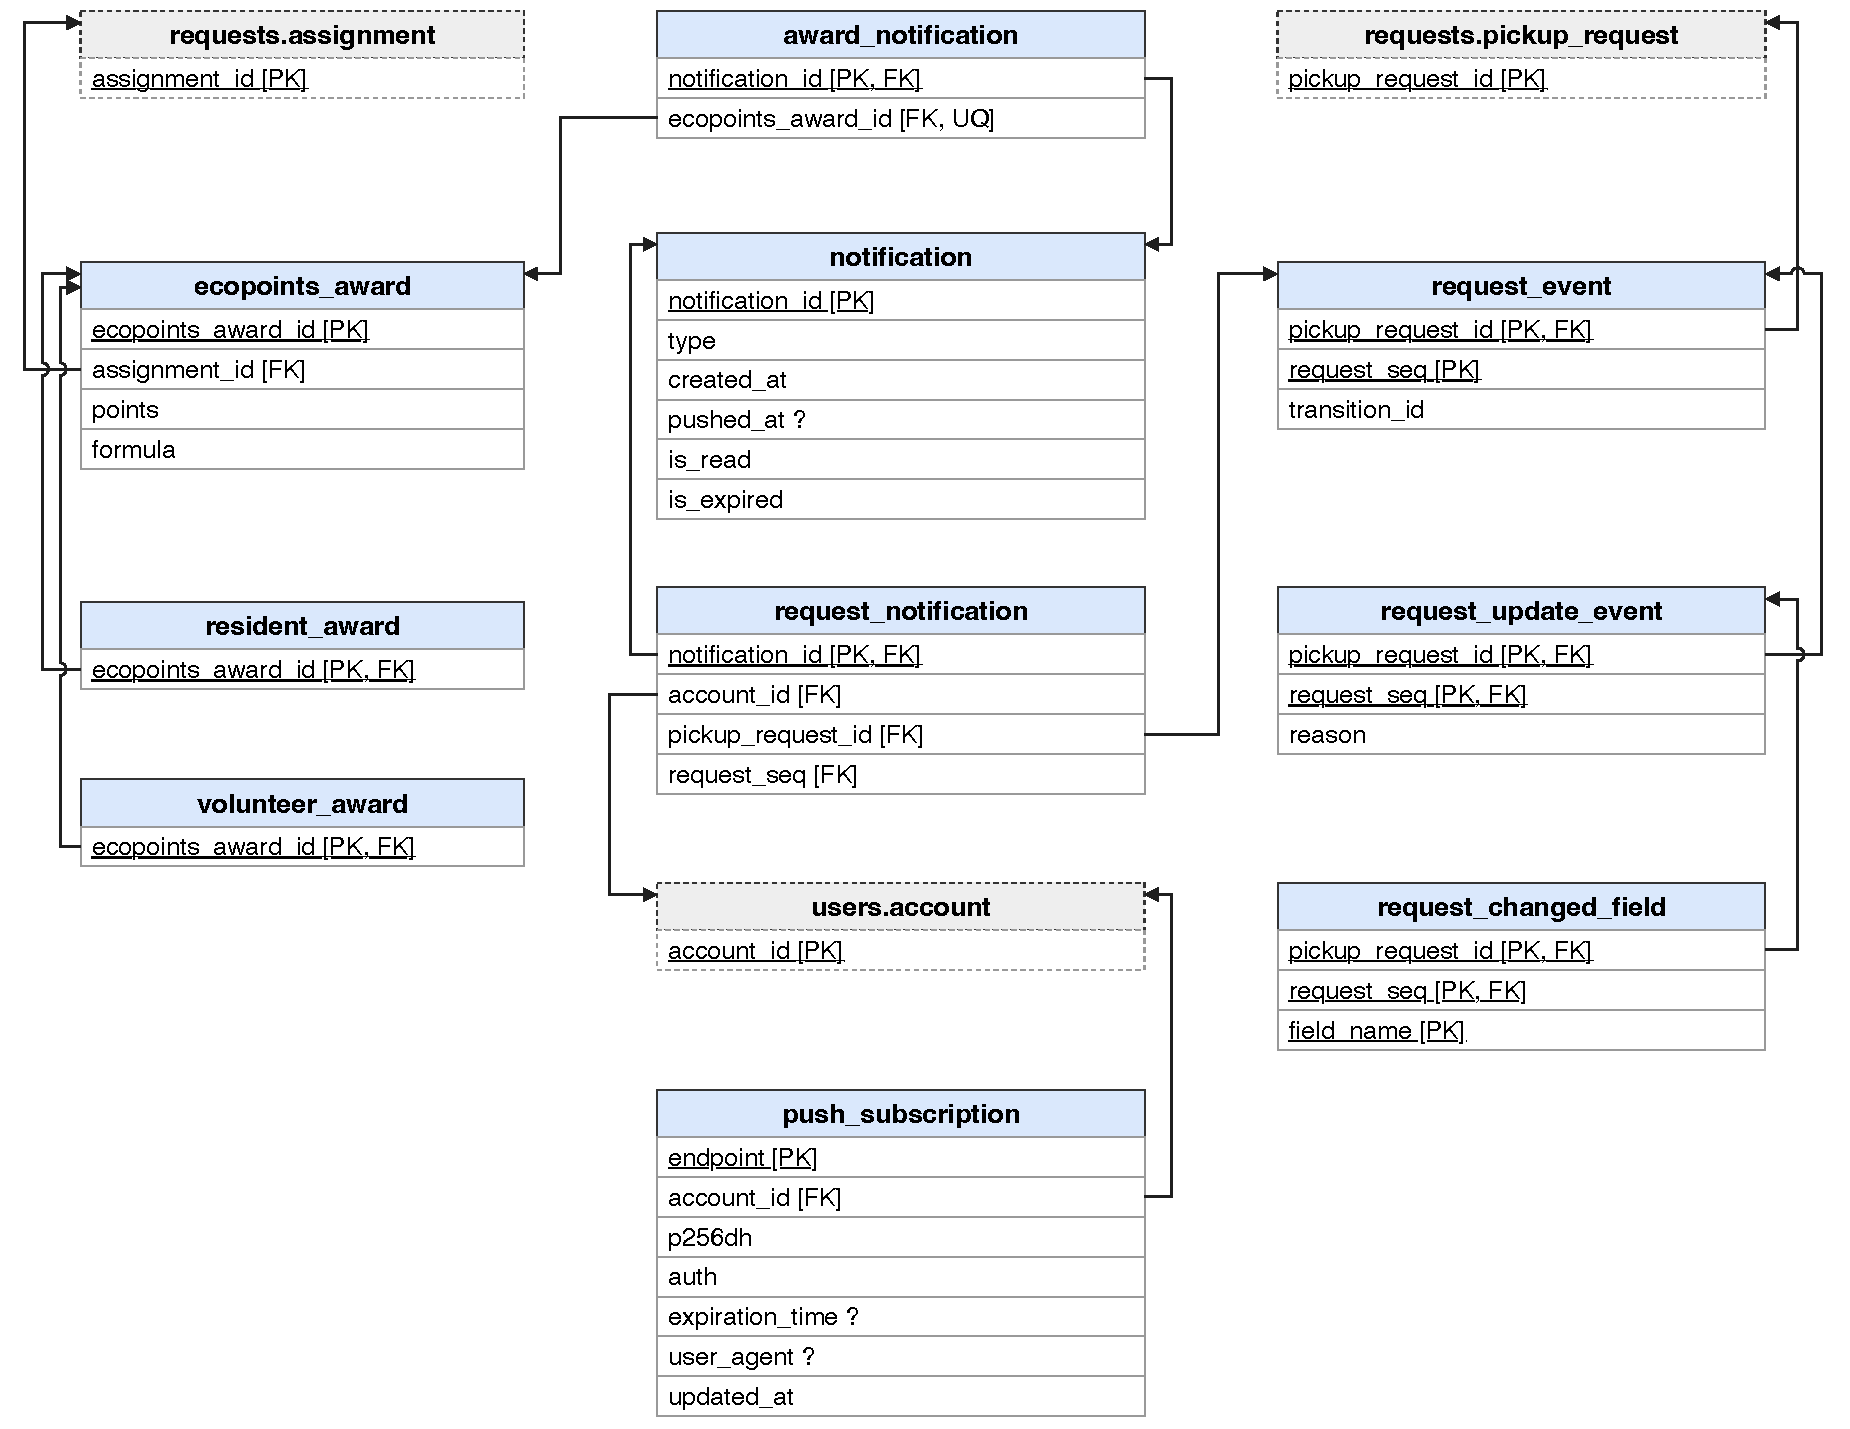
\includegraphics[width=0.97\linewidth]{figures/rel-rewards-notifications.pdf}
\caption{Relational diagram: \texttt{rewards} and \texttt{notifications} schemas}
\label{fig:rel-rewards}
\end{figure}

%----------------------------------------------------------------------
\section{Normalization}
\label{sec:normalization}
\subsection{Functional Dependencies}
In every relation with a single-column primary key, that key determines all other columns. Candidate keys named in Section~\ref{sec:logical} do the same. Table~\ref{tab:fd} lists the dependencies that matter for the composite keys and the design decisions below.

\begin{table}[!ht]
\centering\small
\caption{Functional dependencies relevant to normalization}
\label{tab:fd}
\begin{tabularx}{\linewidth}{@{}Y@{}}
\toprule
(\path{pickup_request_id}, \path{changed_at}) $\rightarrow$ status, reason \\
(\path{pickup_request_id}, \path{request_seq}) $\rightarrow$ \path{transition_id} \quad (in \path{request_event}) \\
(\path{pickup_request_id}, \path{request_seq}) $\rightarrow$ reason \quad (in \path{request_update_event}) \\
\path{pickup_request_id} $\rightarrow$ \path{terms_acceptance_id}; \quad \path{terms_acceptance_id} $\rightarrow$ \path{account_id} \\
\path{assignment_id} $\rightarrow$ \path{pickup_window_id}; \quad \path{pickup_window_id} $\rightarrow$ \path{pickup_request_id} \\
\path{notification_id} $\rightarrow$ (\path{pickup_request_id}, \path{request_seq}) $\rightarrow$ \path{transition_id} \quad (for request notifications) \\
\path{category_id} $\rightarrow$ name, \path{waste_type}, \path{standard_weight_kg} \\
\bottomrule
\end{tabularx}
\end{table}

The other three composite-key relations, \path{volunteer_preferred_postal_code}, \path{facility_accepts} and \path{request_changed_field}, consist only of key columns.

\subsection{First Normal Form}
1NF requires one value in each column of each row. Repeating information has its own relation: one row for each preferred postal code, facility and category pair, pickup window, status change and changed field. Composite names and addresses are separate columns. An earlier notification design held event details and a list of changed fields in one JSON value. We separated it into \path{request_event}, \path{request_update_event} and \path{request_changed_field}. Notes, terms content and formula text stay as single values because the system always uses each one as a whole.

\subsection{Second Normal Form}
2NF also requires that each non-key column depend on the whole of every candidate key. Nineteen relations have only single-column candidate keys, so they cannot have a partial dependency. The other six have composite primary keys. Three contain only key columns. In \path{status_change}, \path{request_event} and \path{request_update_event}, both parts of the key are needed: timestamps and sequence numbers can repeat across requests, and one request has many of them. As a contrast, adding a facility name to \path{facility_accepts}(\path{facility_id}, \path{category_id}) would make it depend on \path{facility_id} alone. That partial dependency is why names stay in \path{recycling_facility} and \path{item_category}.

\subsection{Third Normal Form}
3NF also removes cases where a non-key column determines another non-key column. Table~\ref{tab:3nf} shows the four decisions where this mattered. Each remaining join follows a required foreign key to exactly one parent row, so the removed value is recovered without losing or duplicating rows.

\begin{table}[!ht]
\centering\small
\caption{Third normal form decisions}
\label{tab:3nf}
\begin{tabularx}{\linewidth}{@{}L{0.18\linewidth}YY@{}}
\toprule
Case & Dependency to avoid & Final design \\
\midrule
Request owner & Storing the resident in the request gives request $\rightarrow$ acceptance $\rightarrow$ account. One acceptance can cover several requests (BR43). & The request stores only \path{terms_acceptance_id}; the owner is reached by a join. \\
Assignment & Storing the request or volunteer gives assignment $\rightarrow$ window $\rightarrow$ request, and assignment $\rightarrow$ acceptance $\rightarrow$ account. & \path{assignment} stores only the window and acceptance. \\
Award recipient & A stored recipient repeats what the assignment and earned role already determine. & The role is the row in \path{resident_award} or \path{volunteer_award}; the recipient is derived. \\
Notification facts & Copying event facts gives notification $\rightarrow$ event $\rightarrow$ transition and reason. & Request notifications reference the event key. Award notifications derive the recipient from the award. \\
\bottomrule
\end{tabularx}
\end{table}

With these dependencies, the 25 relations satisfy 1NF, 2NF and 3NF.

\subsection{Historical Facts}
A request keeps its pickup address and estimated weight, and an award keeps its points and formula. These are not redundant copies. A resident's address or a category's standard weight can change later, while the earlier request must keep the values that applied to it (BR31, BR34, BR41). For example, (\path{category_id}, quantity) does not determine \path{estimated_weight_kg} across the request history.

%----------------------------------------------------------------------
\section{Physical Implementation and Data}
\label{sec:physical}
\subsection{Schemas and SQL Files}
The database targets PostgreSQL 16~\cite{postgres}. All results reported here come from commit \texttt{\evidencecommit} of our repository~\cite{repo}. Tables are defined in \path{db/init/005_user_tables.sql}, \path{010_request_tables.sql}, \path{012_reward_tables.sql} and \path{040_notification_tables.sql}. The schema boundaries follow which service writes each table. Foreign keys cross schemas where requests use terms acceptances, awards use assignments, and notifications use accounts, requests and awards.

The schema declares primary keys, 30 foreign keys, unique constraints and \texttt{CHECK} constraints, and its required columns have no \texttt{DEFAULT} values. It has two additional indexes, on \path{account_id} in \path{push_subscription} and in \path{request_notification}. The course setup also loads 36 PL/pgSQL functions into the \path{requests} schema. It has no triggers.

\subsection{Where Rules Are Enforced}
Keys and column constraints cannot express rules that involve several rows or the current time. Table~\ref{tab:enforcement} states where each group of rules is enforced.

\begin{table}[!ht]
\centering\small
\caption{Enforcement of business rules}
\label{tab:enforcement}
\begin{tabularx}{\linewidth}{@{}L{0.23\linewidth}Y@{}}
\toprule
Enforced by & Rules \\
\midrule
Keys and unique constraints & References; one delivery per assignment; one delivery per evidence photo; one replacement per missed request; one notification per award. \\
\texttt{CHECK} and \texttt{NOT NULL} & Required values and formats; closed value sets; positive quantities, weights and points; age of at least 18 at registration; order of assignment timestamps; a Delivered ending requires collection. \\
Request Service PL/pgSQL functions & Write functions lock the rows involved and check an action before writing. This includes time-dependent rules, such as future windows. Before commit, \path{requests.check_request()} rechecks request-level rules, including one to three distinct active windows within 30 days, at most one unfinished assignment, an eligible delivery facility, current terms at acceptance and a valid rescheduling link. \\
User Service transactions and validation & Accounts are created with at least one role; at most three preferred postal codes; no address change while a request is Open or Assigned; no deactivation with active work. \\
Reward Service transactions & Each new award gets exactly one role row; a repeat award for the same assignment and role is skipped; no cancellation award to a resident who is also the volunteer. \\
Notification Service transactions & Each new notification is saved with one source row; award notifications are saved only for stored awards and active accounts. \\
Reference seed data only & Every facility accepts a category and every category has a facility (BR66). No constraint or application code checks this. \\
\bottomrule
\end{tabularx}
\end{table}

Only the first two rows apply to every write. The others apply when changes go through the functions and services, so a privileged user writing SQL directly could break them.

\subsection{Population}
Because foreign keys cross schemas, the scripts run in this order: the numbered table and reference scripts in \path{db/init/}, the Request functions in \path{db/request/}, the sample requests and the course scenario. \path{011_request_seed.sql} loads item categories, facilities and the categories each facility accepts. \path{031_user_seed.sql} loads versions 2 and 3 of the terms. \path{backend/test/request/seed.sql} adds version 1, accounts, requests, windows, status history, assignments and deliveries with dates relative to load time, and checks each request with \path{check_request()}. \path{backend/test/ensf608/scenario.sql} adds awards, subscriptions, events and notifications. Table~\ref{tab:counts} gives the resulting row counts; all 25 course tables are populated.

\begin{table}[!ht]
\centering\small
\caption{Rows in the 25 course tables after seeding (215 in total)}
\label{tab:counts}
\begin{tabular}{@{}lr@{\hspace{2.5em}}lr@{}}
\toprule
Table & Rows & Table & Rows \\
\midrule
\path{account} & 7 & \path{recycling_facility} & 3 \\
\path{resident} & 4 & \path{facility_accepts} & 11 \\
\path{volunteer} & 4 & \path{delivery} & 2 \\
\path{volunteer_preferred_postal_code} & 5 & \path{ecopoints_award} & 5 \\
\path{terms_document} & 3 & \path{resident_award} & 2 \\
\path{terms_acceptance} & 26 & \path{volunteer_award} & 3 \\
\path{item_category} & 9 & \path{push_subscription} & 2 \\
\path{photo} & 4 & \path{notification} & 13 \\
\path{pickup_request} & 11 & \path{request_notification} & 8 \\
\path{pickup_window} & 13 & \path{award_notification} & 5 \\
\path{status_change} & 29 & \path{request_event} & 33 \\
\path{assignment} & 8 & \path{request_update_event} & 3 \\
 & & \path{request_changed_field} & 2 \\
\bottomrule
\end{tabular}
\end{table}

The accounts include one with both roles and a volunteer with no preferred postal code. The 11 requests in Table~\ref{tab:requests} cover all seven statuses, including a missed request (0007) and its replacement (0008).

\begin{table}[!ht]
\centering\small
\caption{Sample pickup requests (identified by the last four characters of their IDs)}
\label{tab:requests}
\begin{tabular}{@{}lllrrll@{}}
\toprule
ID & Resident & Category & Qty & Est. kg & Postal code & Status \\
\midrule
0001 & resident1 & Computers/Laptops & 2 & 5.00 & T2P1J9 & Open \\
0002 & resident2 & Computers/Desktops & 1 & 8.00 & T2N1N4 & Assigned \\
0003 & resident3 & Phones & 4 & 0.80 & T2T4M3 & Collected \\
0004 & resident1 & Computers/Laptops & 2 & 5.00 & T2P1J9 & Delivered \\
0005 & resident2 & Monitors & 1 & 5.00 & T2N1N4 & Cancelled \\
0006 & resident1 & Televisions & 1 & 12.00 & T2P1J9 & Expired \\
0007 & resident3 & Printers & 1 & 6.00 & T2T4M3 & Missed \\
0008 & resident3 & Printers & 1 & 6.00 & T2T4M3 & Open \\
0009 & both1 & Phones & 3 & 0.60 & T2P1J9 & Delivered \\
000a & resident1 & Cables and Chargers & 5 & 1.50 & T2P1J9 & Open \\
000b & resident1 & Small Appliances & 1 & 3.00 & T2P1J9 & Open \\
\bottomrule
\end{tabular}
\end{table}

%----------------------------------------------------------------------
\section{Database Operations and Queries}
\label{sec:operations}
The file \path{operations.sql} contains 27 operations grouped by the course categories: the required 25 and two further queries, G3 and C2, for questions in our proposal. Table~\ref{tab:categories} shows the coverage. A helper view, \path{request_current_status}, which derives each request's owner and latest status, is not counted. Write examples and procedure calls run in transactions that are rolled back. The file creates the view and procedures in a helper schema and removes that schema at the end.

\begin{table}[!ht]
\centering\small
\caption{Coverage of the required operation categories}
\label{tab:categories}
\begin{tabular}{@{}lccl@{}}
\toprule
Category & Required & Provided & Identifiers \\
\midrule
INSERT & 2 & 2 & I1, I2 \\
UPDATE & 2 & 2 & U1, U2 \\
DELETE & 2 & 2 & D1, D2 \\
SELECT with filtering & 4 & 4 & F1--F4 \\
SELECT with ORDER BY, DISTINCT or LIMIT & 2 & 2 & O1, O2 \\
Aggregate functions & 3 & 3 & A1--A3 \\
GROUP BY, at least one with HAVING & 2 & 3 & G1--G3 \\
INNER JOIN & 3 & 3 & J1--J3 \\
LEFT or RIGHT JOIN & 2 & 2 & L1, L2 \\
Joins with aggregates, filtering or grouping & 1 & 2 & C1, C2 \\
Stored procedures & 2 & 2 & P1, P2 \\
\midrule
Total & 25 & 27 & \\
\bottomrule
\end{tabular}
\end{table}

\subsection{Operation Catalogue}
Table~\ref{tab:catalogue} gives the purpose of each operation and its result on the sample data. The notification operations cover request notifications only, while the application's notification service also handles award notifications. Results that depend on dates change with the time of loading. The complete SQL is in \path{operations.sql}, and the complete output of one run on PostgreSQL 16.16 is in \path{results/operations.txt}.

{\small
\begin{longtable}{@{}lL{0.47\linewidth}L{0.42\linewidth}@{}}
\caption{Operations, purposes and results}\label{tab:catalogue}\\
\toprule
ID & Purpose & Result on sample data \\
\midrule
\endfirsthead
\toprule
ID & Purpose & Result on sample data \\
\midrule
\endhead
\bottomrule
\endfoot
I1 & Register a resident: account, role and terms acceptance in one transaction & Three rows inserted; the acceptance refers to terms version 3 \\
I2 & Save a browser push subscription, updating it if the endpoint exists & One row saved \\
U1 & Change the public name of an active account & One row updated \\
U2 & Replace an Open request's windows under a row lock & Two windows retired and one added; sequence now 3; request checks passed \\
D1 & Remove a volunteer's preferred postal code & One row deleted; two codes remain \\
D2 & Delete expired notifications, source rows first & One notification and its source row deleted; 12 remain \\
F1 & List a volunteer's preferred postal codes & 3 codes \\
F2 & Find a resident's Open or Assigned requests & 1 request (0002, Assigned) \\
F3 & Find Open requests in a volunteer's postal codes (expiry not checked) & 4 requests \\
F4 & List active windows dated today to seven days ahead & 6 windows \\
O1 & List categories by waste type and name, with standard weights & 9 categories \\
O2 & Show a resident's two newest unexpired request notifications & 2 rows \\
A1 & Total delivered requests and their estimated weight & 2 requests, 5.60 kg \\
A2 & Summarize the weight of Open requests & 4 requests; average 3.88, minimum 1.50, maximum 6.00 kg \\
A3 & Count a resident's unread, unexpired request notifications & 1 \\
G1 & Total all requests and estimated weight by waste type & 6 types; computers highest at 18.00 kg \\
G2 & Find categories requested at least twice & 3 categories \\
G3 & Count expired requests by Calgary month & November 2026: 1 \\
J1 & Find facilities that accept phones (3 tables) & 2 sample facilities \\
J2 & Show a resident's requests with category and current status & 5 requests \\
J3 & List unfinished assignments with window and collection state (5 tables) & 2 assignments \\
L1 & Show a volunteer's assignments, with delivery facility if any & 2 rows, one without a delivery \\
L2 & List all volunteers with preferred codes, including those with none & 6 rows; \path{volunteer3} has no code \\
C1 & Total EcoPoints by account and role & 5 rows; highest 26.00 points \\
C2 & Total delivered requests, items and weight by category (5 tables) & Phones: 3 items, 0.60 kg; laptops: 2 items, 5.00 kg \\
P1 & Procedure: mark all of an account's request notifications read (input parameter) & One unread notification became read \\
P2 & Procedure: mark one notification read if the account owns it (input and output parameters) & Found for the owner; not found, and unchanged, for another account \\
\end{longtable}
}

\needspace{28\baselineskip}
\subsection{Questions from the Proposal}
Our proposal posed six questions. Table~\ref{tab:questions} shows how the final operations answer them.

\begin{table}[!ht]
\centering\small
\caption{Proposal questions and final operations}
\label{tab:questions}
\begin{tabularx}{\linewidth}{@{}L{0.37\linewidth}lY@{}}
\toprule
Proposal question & Operations & Coverage \\
\midrule
Which Open, unexpired requests are in a selected postal code area, with what items and offered slots? & F3 & In part: matches a volunteer's saved codes and returns categories, without slots or an expiry filter. The application's list function applies those but is not one of the 27. \\
Which requests are assigned to a volunteer, with what slots and statuses? & J3, L1 & In part: J3 gives windows and collection state for unfinished assignments; L1 gives one volunteer's outcomes without windows. \\
How many requests expired each month, including those later renewed? & G3 & Answered for expiry. Renewal does not exist in the final system. \\
How much e-waste was diverted to proper recycling? & A1 & Answered with estimated weight. \\
What are the delivered quantities by item category? & C2 & Answered. \\
What is the current status of a particular request? & J2 & In part: the helper view derives current status and J2 lists it for one resident's requests; no counted operation selects a single request. \\
\bottomrule
\end{tabularx}
\end{table}

\subsection{Selected Operations and Output}
The following excerpts are taken from the SQL file and its saved output. They show grouping with \texttt{HAVING}, a \texttt{LEFT JOIN}, a query that combines five tables with aggregates, and a procedure with input and output parameters. Table names are unqualified because the file sets the schema search path.

\needspace{15\baselineskip}
\textbf{G2: categories requested at least twice}
\lstinputlisting[language=SQL]{sql/G2.sql}
\lstinputlisting{sql/G2-result.txt}

\needspace{20\baselineskip}
\textbf{L1: a volunteer's history, keeping assignments without a delivery}
\lstinputlisting[language=SQL]{sql/L1.sql}
\lstinputlisting{sql/L1-result.txt}

\needspace{18\baselineskip}
\textbf{C2: delivered items and estimated weight by category}
\lstinputlisting[language=SQL]{sql/C2.sql}
\lstinputlisting{sql/C2-result.txt}

\needspace{30\baselineskip}
\textbf{P2: mark a notification read only for its owner}
\lstinputlisting[language=SQL]{sql/P2.sql}
The first call returned \texttt{p\_found = t} and marked the notification read. The second, for a notification owned by another resident, returned \texttt{p\_found = f} and left it unread.

%----------------------------------------------------------------------
\section{Database Testing}
\label{sec:testing}
\subsection{Method}
The test script \path{backend/test/ensf608/application.sql} runs on the seeded database. Each case raises an error if its expectation fails, and rejection cases check that PostgreSQL raises the expected error. The changes run inside a transaction that is rolled back, so the script can be repeated. A final case checks the rollback.

\subsection{Test Cases and Results}
Table~\ref{tab:tests} lists the nine cases and their results.
{\small
\begin{longtable}{@{}lL{0.48\linewidth}L{0.31\linewidth}l@{}}
\caption{Database test cases}\label{tab:tests}\\
\toprule
Case & Action & Expected & Result \\
\midrule
\endfirsthead
\toprule
Case & Action & Expected & Result \\
\midrule
\endhead
\bottomrule
\endfoot
APP01 & Count course tables, columns, primary keys and validated foreign keys in the catalogue & 25, 100, 25 and 30 & Pass \\
APP02 & Join delivery to assignment, window and request & 2 deliveries, 5.60 kg & Pass \\
APP03 & Check facility coverage for phones and for the first facility & 2 facilities; 8 categories & Pass \\
APP04 & Insert an award notification and join it to its award & Insert succeeds; 13 points & Pass \\
APP05 & Point an award notification at an unknown award & Foreign key error 23503 & Pass \\
APP06 & Insert a duplicate facility and category pair & Unique violation 23505 on the primary key & Pass \\
APP07 & Set a quantity to zero; remove a required public name & Errors 23514 and 23502 & Pass \\
APP08 & Mark a notification read, then delete it & Both succeed; award remains & Pass \\
APP09 & Check the data after rollback & Original notification restored & Pass \\
\end{longtable}
}

All nine cases passed on two consecutive runs. The saved log, \path{results/application.txt}, is from PostgreSQL 18.6. The suite also passed twice on PostgreSQL 16.16 in the run that produced the saved query output.

\subsection{Coverage and Checks of the Operations}
The suite asserts the database structure (APP01), retrieval across related tables (APP02, APP03), data changes (APP04, APP08) and rejection of invalid data by a foreign key, a composite primary key, a \texttt{CHECK} constraint and \texttt{NOT NULL} (APP05 to APP07). The 27 operations and both procedures also ran without error, with their output saved. Apart from the cases above, their results have no automated assertions.

Further checks were made on PostgreSQL 16.16 when G3 and C2 were added. C2 matched a separate query based on status history, and its totals matched A1. In a rolled-back test, G3 placed rows on either side of a Calgary month boundary in the correct months and counted a repeated request once. The 215 course rows and the two Notification Service procedures, loaded additionally for this comparison, were the same before and after running \path{operations.sql}.

The suite has these gaps. It has no rejection case for the rules in the lower rows of Table~\ref{tab:enforcement}, such as a second unfinished assignment or an ineligible delivery facility. It does not separately test an alternate unique key or the age rule, and it does not test the two course procedures with assertions. The repository's service-level tests are not part of this evidence.

%----------------------------------------------------------------------
\section{Setup and Use}
\label{sec:setup}
The course database needs Bash and PostgreSQL 16 or later. Use a separate, disposable PostgreSQL server, because some setup scripts create database roles. Set \path{PGHOST}, \path{PGPORT} and \path{PGUSER} to an account that can create databases, schemas and roles. From the repository root, create and populate the database:
\begin{lstlisting}[language=bash]
createdb ecocollect_608_test || exit 1
for file in db/init/{005,010,011,012,031,040}_*.sql db/request/*.sql \
    backend/test/request/seed.sql backend/test/ensf608/scenario.sql; do
  psql -X -v ON_ERROR_STOP=1 -d ecocollect_608_test -f "$file" || exit 1
done
\end{lstlisting}
\needspace{9\baselineskip}
Run the operations and then the tests soon after loading, because the sample dates are relative to load time:
\begin{lstlisting}[language=bash]
psql -X -a -v ON_ERROR_STOP=1 -d ecocollect_608_test \
  -f "docs/Final Submission/ENSF608/5. Database operations and queries/operations.sql"
psql -X -v ON_ERROR_STOP=1 -d ecocollect_608_test \
  -f backend/test/ensf608/application.sql
\end{lstlisting}
If a script fails, correct the cause and start again with a new database name, using that name in all later commands. To explore the data, connect with \texttt{psql -d ecocollect\_608\_test}; the command \texttt{\textbackslash dt users.*} lists the tables in one schema, and ordinary \texttt{SELECT} statements read them. The repository's \path{README.md} and \path{db/README.md} describe how to run the full application with Docker Compose.

%----------------------------------------------------------------------
\section{Individual Team Member Contributions}
\label{sec:contributions}
Table~\ref{tab:contributions} summarizes contributions that can be traced to commits and pull requests (PRs) in the repository. It covers committed work, not discussion, review or presentation preparation. Several files were changed by more than one member after their first version.

{\small
\begin{longtable}{@{}L{0.19\linewidth}L{0.55\linewidth}L{0.20\linewidth}@{}}
\caption{Individual contributions}\label{tab:contributions}\\
\toprule
Member & Contribution & Pull requests \\
\midrule
\endfirsthead
\toprule
Member & Contribution & Pull requests \\
\midrule
\endhead
\bottomrule
\endfoot
Krunaliben Patel (\texttt{Krunali49}) & Logical model and normalization documents; later refinements of the conceptual diagram; User Service tables and outbox; alignment of the physical schema with the model; the course test suite and scenario data; updates to the operations and saved results. & 172, 185, 195, 196, 198, 284, 295, 500, 516 \\
\addlinespace
Jasdeep Singh Malhotra (\texttt{cingh-jasdeep}) & First conceptual diagram; Request Service schema, reference data, PL/pgSQL functions and request test data; replay and time-rule corrections; extension of notification event storage. & 106, 296, 444, 465, 501 \\
\addlinespace
Danny Dufau (\texttt{dannydufau}) & PostgreSQL in Docker Compose; the initial catalogue of operations, including the helper view and procedures; Notification Service tables and procedures. & 27, 399, 443 \\
\addlinespace
Saad Ahmad Malik (\texttt{saada865}) & Reward Service award tables and database operations; Cleanup Service schema for expiry jobs and events. & 364, 367 \\
\addlinespace
Satyam Bhanot (\texttt{satyambhanot}) & First version of the shared contracts; further Docker Compose services; Calgary time-zone test corrections; setup documentation; notification database changes and review fixes; small changes within the reward and cleanup work; version 3 terms seed; queries G3 and C2 with regenerated output. & 33, 43, 51, 364, 367, 399, 443, 501, 502, 511, 521 \\
\addlinespace
Vedant Patel (\texttt{vedantp-14}) & Web application pages and data fetching that use the database-backed service interfaces. & 176, 183, 200, 297--303, 321--328, 363, 371--386, 390--393 \\
\end{longtable}
}

%----------------------------------------------------------------------
\section{Limitations and Conclusion}
\label{sec:conclusion}
The main limitations of the final database are these. Several rules depend on functions, service transactions or seed data instead of declarative constraints (Table~\ref{tab:enforcement}). The recycling facilities are placeholders, and real facilities and their accepted categories would need to be confirmed before use. Weights are estimates. The sample data set is small, so no performance conclusions can be drawn from it. Automated course tests cover a limited set of constraints, as described in Section~\ref{sec:testing}.

Within these limits, the database carries the design consistently from a 20-entity conceptual model to 25 relations in third normal form and their PostgreSQL implementation. The setup scripts build and populate it, the 27 operations run against it, and the nine database tests pass. It records what residents offer, who collects it, where it is delivered and which requests go uncollected, which is the information EcoCollect needs to support its part of SDG 12.

%----------------------------------------------------------------------
\section{Academic Integrity}
% Copied word for word from the team's Word report.
\subsection{Generative AI Usage Disclosure}
During the development of EcoCollect and the preparation of this report, our team used generative AI tools (including Google Gemini) as supporting resources to seek guidance, understand database concepts, explore possible solutions, assist with SQL/documentation structuring and formatting, and receive verification feedback. AI supported our learning rather than replacing our own understanding and efforts. The team reviewed, executed against PostgreSQL, understood, and adapted all AI-assisted material to meet project requirements instead of directly copying generated content.


%----------------------------------------------------------------------
\phantomsection
\addcontentsline{toc}{section}{References}
\begin{thebibliography}{9}
\bibitem{calgary} City of Calgary, ``Electronics recycling for residents.'' [Online]. Available: \url{https://www.calgary.ca/waste/residential/electronics-recycling-depots.html}. Accessed 27 November 2026.
\bibitem{sdg12} United Nations, ``Goal 12: Ensure sustainable consumption and production patterns.'' [Online]. Available: \url{https://sdgs.un.org/goals/goal12}. Accessed 27 November 2026.
\bibitem{postgres} PostgreSQL Global Development Group, ``PostgreSQL 16 documentation.'' [Online]. Available: \url{https://www.postgresql.org/docs/16/}. Accessed 27 November 2026.
\bibitem{repo} Group 9, ``EcoCollect source repository,'' commit \texttt{\evidencecommit}. [Online]. Available: \url{https://github.com/dannydufau/ecocollect}.
\end{thebibliography}

%----------------------------------------------------------------------
\clearpage
\appendix
\section{Business Rules}
\label{app:rules}
Table~\ref{tab:rules} lists the rules recorded in the conceptual diagram. We corrected one typing error in BR32 and removed examples from BR37 that no longer matched the item categories. Codes beginning with FR or NFR refer to the project's functional and non-functional requirements.
{\small
% Generated from the business-rule note in ER-Diagram.drawio.
\begin{longtable}{@{}p{0.07\linewidth}>{\raggedright\arraybackslash}p{0.89\linewidth}@{}}
\caption{Business rules}\label{tab:rules}\\
\toprule
Rule & Statement \\
\midrule
\endfirsthead
\toprule
Rule & Statement \\
\midrule
\endhead
\bottomrule
\endfoot
BR1 & Every ACCOUNT has at least one role (RESIDENT, VOLUNTEER or both). A second role is activated on the same account, never a duplicate account. \\
\addlinespace[2pt]
BR2 & Registration and role activation record a TERMS\_ACCEPTANCE, so every account has at least one. Related type values are AT\_RESIDENT\_REGISTRATION\_OR\_ACTIVATION and AT\_VOLUNTEER\_REGISTRATION\_OR\_ACTIVATION. \\
\addlinespace[2pt]
BR3 & Account\_ID is unique across all accounts. \\
\addlinespace[2pt]
BR4 & Account\_ID, First\_Name, Last\_Name, Public\_Name, and Date\_Of\_Birth are required for all accounts. \\
\addlinespace[2pt]
BR5 & Address is required for a RESIDENT account. \\
\addlinespace[2pt]
BR6 & The account holder must be 18 or older, and Date\_Of\_Birth cannot be in the future. Age is derived from Date\_Of\_Birth. \\
\addlinespace[2pt]
BR7 & Postal\_Code matches \texttt{\textasciicircum T[0-9][A-Z][0-9][A-Z][0-9]\$} (for example T2P1J9). The application validates that the address is in Calgary. \\
\addlinespace[2pt]
BR8 & A RESIDENT cannot change their profile address while they have a pickup request that is Open or Assigned. \\
\addlinespace[2pt]
BR9 & A VOLUNTEER saves 0 to 3 distinct Preferred\_Postal\_Code values. Saved codes trigger matching notifications unless the account is deactivated; with none saved, no new-request match notifications are generated for that Volunteer. \\
\addlinespace[2pt]
BR10 & A NOTIFICATION belongs to exactly one account and is used to deliver in-app and push notifications. \\
\addlinespace[2pt]
BR11 & Each ECOPOINTS\_AWARD is earned through exactly one role: by a VOLUNTEER or by a RESIDENT. A delivery creates a volunteer award and a resident award. When a volunteer delivers their own request, their account receives both. A resident's cancellation outside the cancellation window creates a volunteer award only. The cancellation window is the period at least 24 hours before the start of the assignment's pickup window. No cancellation award is created when the volunteer is also the request's resident. \\
\addlinespace[2pt]
BR12 & Combined\_Ecopoints (ACCOUNT) is derived: the sum of Points over all ECOPOINTS\_AWARDs the account has earned in either role, as a RESIDENT and as a VOLUNTEER, including delivery and cancellation awards. \\
\addlinespace[2pt]
BR13 & A RESIDENT owns the requests they create, and the owner never changes. Only the owning resident can confirm a collection while the request is Assigned. \\
\addlinespace[2pt]
BR14 & Every ASSIGNMENT belongs to exactly one VOLUNTEER, and a volunteer can accept a request created by their own account. \\
\addlinespace[2pt]
BR15 & Public profiles show only Public\_Name, Account\_ID, roles, ecopoints and member since (Created\_At). Legal name, email, birth date, address and PICKUP\_REQUEST details (quantity, item category, etc.) stay private. \\
\addlinespace[2pt]
BR16 & Every PICKUP\_REQUEST has at least one STATUS\_CHANGE; the first one records Open when the request is created. \\
\addlinespace[2pt]
BR17 & A STATUS\_CHANGE is added each time the request status changes, including expiry and reopening, and is never edited. Reason is optional and explains the change, for example, expired or missed pickup. \\
\addlinespace[2pt]
BR18 & STATUS\_CHANGE is weak: it is identified by its PICKUP\_REQUEST plus Changed\_At. Status is one of Open, Assigned, Collected, Delivered, Cancelled, Expired, Missed. \\
\addlinespace[2pt]
BR19 & An ASSIGNMENT links one VOLUNTEER, one PICKUP\_REQUEST and one PICKUP\_WINDOW, which must be one of the windows that request offers. \\
\addlinespace[2pt]
BR20 & A PICKUP\_REQUEST has at most one ASSIGNMENT that hasn't ended (Ended\_At empty) at a time. Ended assignments are kept for history. \\
\addlinespace[2pt]
BR21 & ASSIGNMENT: Collected\_At is set when the owning resident confirms collection. \\
\addlinespace[2pt]
BR22 & An ASSIGNMENT can be cancelled or reported missed only before Collected\_At is set. A missed pickup can be reported only after the selected window ends. A resident can cancel the request or its assignment only until the selected window ends; after that they confirm collection or report a missed pickup. A volunteer can cancel any time before Collected\_At is set. If an assignment is cancelled by the resident or the volunteer, the request returns to Open if valid future windows remain, otherwise it becomes Expired; the resident may offer new windows. If a missed pickup is reported, the request becomes Missed, a final status, and the resident may reschedule, which creates a new PICKUP\_REQUEST linked to the missed one. \\
\addlinespace[2pt]
BR23 & ASSIGNMENT: Ended\_At and End\_Reason are set together. End\_Reason is one of Delivered, Volunteer\_Cancelled, Resident\_Cancelled, Missed\_Pickup. \\
\addlinespace[2pt]
BR24 & ASSIGNMENT: Status is derived: "Active" if Collected\_At and Ended\_At are empty, "Collected" if only Collected\_At is set, otherwise the End\_Reason. \\
\addlinespace[2pt]
BR25 & A DELIVERY is recorded only for a collected ASSIGNMENT, by its volunteer. An ASSIGNMENT has at most one DELIVERY. \\
\addlinespace[2pt]
BR26 & DELIVERY: Delivered\_At cannot be earlier than Collected\_At. \\
\addlinespace[2pt]
BR27 & A DELIVERY is recorded only when the facility accepts the items; items a facility refuses are handled outside the app. \\
\addlinespace[2pt]
BR28 & A DELIVERY can only go to a facility that accepts the request's ITEM\_CATEGORY. \\
\addlinespace[2pt]
BR29 & Each assignment requires exactly one acknowledgment of the terms, a TERMS\_ACCEPTANCE of Type AT\_VOLUNTEER\_ACCEPTANCE, made by the assignment's Volunteer. \\
\addlinespace[2pt]
BR30 & PICKUP\_REQUEST: Quantity is a positive integer. \\
\addlinespace[2pt]
BR31 & PICKUP\_REQUEST: Estimated\_Weight\_Kg = Quantity * Standard\_Weight\_Kg (2 decimals). It's computed by the system and recalculated on edit (FR06, FR10). Changing Standard\_Weight\_Kg does not update existing requests. \\
\addlinespace[2pt]
BR32 & PICKUP\_REQUEST: A request offers 1--3 windows that don't overlap and start in the future, each with one hourly slot (0-23) based on the starting hour of the day, ending no later than Created\_At + 30 days (FR07). A request can only offer up to 3 active windows (Is\_Active = true) at once. \\
\addlinespace[2pt]
BR33 & PICKUP\_REQUEST: Expires\_At = the start of its last active PICKUP\_WINDOW, recalculated when the active windows change (FR10). Every window ends by Created\_At + 30 days (BR32), so a request never stays Open past 30 days, and reopening doesn't move that limit. Only Open requests expire (FR20). \\
\addlinespace[2pt]
BR34 & PICKUP\_REQUEST: Pickup\_Address is copied from the resident's profile at creation and never changes (FR07, FR10). \\
\addlinespace[2pt]
BR35 & PICKUP\_REQUEST: Only Open requests can be edited (FR10, BR45). \\
\addlinespace[2pt]
BR36 & PICKUP\_WINDOW: Replaced windows are kept with Is\_Active = false, for assignment history. \\
\addlinespace[2pt]
BR37 & ITEM\_CATEGORY: each category has one Name and exactly one Waste\_Type that classifies it. Categories are predefined. \\
\addlinespace[2pt]
BR38 & PICKUP\_REQUEST: A Resident must acknowledge the safety requirements before creating a Pickup Request. The acknowledgment is mandatory and recorded with the request through its TERMS\_ACCEPTANCE. \\
\addlinespace[2pt]
BR39 & RECYCLING\_FACILITY: Facilities are predefined; residents and volunteers can't create them (FR17). \\
\addlinespace[2pt]
BR40 & PUSH\_SUBSCRIPTION: Delete the subscription on device logout or a push response of 404 or 410. On E16 (AccountDeactivated), the Notification Service deletes all subscriptions for that account. \\
\addlinespace[2pt]
BR41 & Volunteer Points = 3 * Quantity + 4 * Estimated\_Weight\_Kg. Resident Points = Volunteer Points / 2, with no rounding. A cancellation award uses the Volunteer formula. Points are stored with 2 decimals. Each ECOPOINTS\_AWARD stores the formula used, as text, when it is created; changing a formula affects only new awards. \\
\addlinespace[2pt]
BR42 & Accounts are deactivated, not deleted. Their history is kept. \\
\addlinespace[2pt]
BR43 & Creating a PICKUP\_REQUEST records a TERMS\_ACCEPTANCE of Type AT\_RESIDENT\_REQUEST\_CREATION for the creating Resident. \\
\addlinespace[2pt]
BR44 & Recording a DELIVERY also sets Ended\_At and End\_Reason = Delivered. Delivered\_At is derived from Ended\_At. \\
\addlinespace[2pt]
BR45 & A request's current Status comes from its latest STATUS\_CHANGE. \\
\addlinespace[2pt]
BR46 & When a request's status changes, the related accounts are notified, except accounts that are deactivated (BR47). \\
\addlinespace[2pt]
BR47 & On E16 (AccountDeactivated), the Notification Service deletes the linked account's notifications and their source rows. \\
\addlinespace[2pt]
BR48 & Each ECOPOINTS\_AWARD creates one NOTIFICATION for the account that earns it, unless that account is deactivated (BR47). Each NOTIFICATION comes from exactly one source: a PICKUP\_REQUEST or an ECOPOINTS\_AWARD. \\
\addlinespace[2pt]
BR49 & A NOTIFICATION about a request is expired when that request moves past the state it describes. Expired notifications are hidden and deleted daily. EcoPoints notifications never expire. They are deleted only with their account (BR47). \\
\addlinespace[2pt]
BR50 & A Missed PICKUP\_REQUEST can be rescheduled once, while reporting the miss, by creating a new PICKUP\_REQUEST that references it. The new request copies the category, quantity, notes and photo; takes the address from the profile; records a new terms acceptance; and has its own Created\_At and Expires\_At. \\
\addlinespace[2pt]
BR51 & An item photo is visible to the request owner and to Volunteers while the request is Open, then to the owner and the assigned Volunteer. A delivery photo is visible only to the owner and the delivering Volunteer. Location metadata is removed before upload. A photo file is deleted only when no request references it. A PICKUP\_REQUEST photo is optional; a DELIVERY photo is required (FR17). \\
\addlinespace[2pt]
BR52 & Is\_Read is set by the user (one notification or all). \\
\addlinespace[2pt]
BR53 & An account can't be deactivated while it owns an Open, Assigned or Collected request or is the volunteer of an assignment that hasn't ended (Ended\_At empty). \\
\addlinespace[2pt]
BR54 & A TERMS\_ACCEPTANCE must reference the current TERMS\_DOCUMENT at the time of acceptance. \\
\addlinespace[2pt]
BR55 & An ASSIGNMENT has at most one ECOPOINTS\_AWARD per role. \\
\addlinespace[2pt]
BR56 & Email is stored only in Firebase, under the account's Account\_ID (the Firebase uid), and Firebase enforces that it's unique. Role membership (RESIDENT, VOLUNTEER) is also copied to Firebase as custom claims. \\
\addlinespace[2pt]
BR57 & Awarded\_At and Type on ECOPOINTS\_AWARD are derived from the assignment. \\
\addlinespace[2pt]
BR58 & NOTIFICATION: Title and Body are derived, never stored. When the notification is sent (SSE and push), Title and Body are built from the event that created it. When the notification list is read, Title and Body are built from the related request, assignment or award. The assignment is the request's latest one for resident notifications, the recipient's latest one on that request for volunteer notifications, and the award's assignment for EcoPoints notifications; this is unambiguous because older notifications expire (BR49). For request notifications, Metadata is derived from REQUEST\_EVENT, its optional REQUEST\_UPDATE\_EVENT and changed-field values. Title and Body never include a street address or photo link (NFR03). \\
\addlinespace[2pt]
BR59 & PICKUP\_REQUEST: Deliverable\_Facilities is derived: the RECYCLING\_FACILITIES that accept the request's ITEM\_CATEGORY. \\
\addlinespace[2pt]
BR60 & Each PHOTO is linked either to one or more requests or to exactly one delivery, never both. \\
\addlinespace[2pt]
BR61 & PICKUP\_REQUEST: Request\_Seq starts at 1 and increases by 1 for every event published about the request (two events from one action get consecutive numbers). A rescheduled request starts at 1. \\
\addlinespace[2pt]
BR62 & Every notification has exactly one source subtype (total and disjoint). Both inherit the notification attributes and recipient relationship. \\
\addlinespace[2pt]
BR63 & REQUEST\_EVENT is identified by its request and Request\_Seq. Transition\_ID identifies an action and may be shared by several events. \\
\addlinespace[2pt]
BR64 & REQUEST\_UPDATE\_EVENT is optional and inherits the event key. Reason is edited or reopened. Changed\_Field lists the fields changed by an edit; reopened events have none. \\
\addlinespace[2pt]
BR65 & Request notification metadata is derived from the event sequence, transition ID, optional update reason and changed fields. Award recipients follow EARNS\_AS\_RESIDENT or EARNS\_AS\_VOLUNTEER (BR11). \\
\addlinespace[2pt]
BR66 & Every RECYCLING\_FACILITY accepts at least one ITEM\_CATEGORY, and every ITEM\_CATEGORY is accepted by at least one RECYCLING\_FACILITY. \\
\addlinespace[2pt]
\end{longtable}

}

\clearpage
\section{Data Dictionary}
\label{app:dictionary}
The columns, types, nullability and keys in Table~\ref{tab:dictionary} were read from the catalogue of a freshly built database. The check descriptions summarize the declared constraints.
{\small
% Generated from the PostgreSQL catalog of a freshly built database.
\begin{longtable}{@{}p{0.34\linewidth}p{0.18\linewidth}p{0.05\linewidth}>{\raggedright\arraybackslash}p{0.325\linewidth}@{}}
\caption{Data dictionary for the 25 course tables}\label{tab:dictionary}\\
\toprule
Column & Type & Null & Key or reference \\
\midrule
\endfirsthead
\toprule
Column & Type & Null & Key or reference \\
\midrule
\endhead
\bottomrule
\endfoot
\multicolumn{4}{@{}l}{\textbf{\texttt{users.account}}} \\*
\path{account_id} & VARCHAR(50) &  & PK \\*
\path{first_name} & VARCHAR(80) &  &  \\*
\path{last_name} & VARCHAR(80) &  &  \\*
\path{public_name} & VARCHAR(80) &  &  \\*
\path{date_of_birth} & DATE &  &  \\*
\path{created_at} & TIMESTAMPTZ &  &  \\*
\path{deactivated_at} & TIMESTAMPTZ & yes &  \\*
\multicolumn{4}{@{}>{\raggedright\arraybackslash}p{0.95\linewidth}@{}}{\textit{Checks:} account\_id has 3 to 50 characters from a--z, 0--9, underscore and hyphen; names are not blank; the holder is at least 18 on the Calgary date of created\_at; deactivated\_at is not before created\_at.} \\
\addlinespace[6pt]
\multicolumn{4}{@{}l}{\textbf{\texttt{users.resident}}} \\*
\path{account_id} & VARCHAR(50) &  & PK, FK to \path{account} \\*
\path{street} & VARCHAR(255) &  &  \\*
\path{postal_code} & CHAR(6) &  &  \\*
\multicolumn{4}{@{}>{\raggedright\arraybackslash}p{0.95\linewidth}@{}}{\textit{Checks:} street is not blank; postal\_code uses the Calgary format.} \\
\addlinespace[6pt]
\multicolumn{4}{@{}l}{\textbf{\texttt{users.volunteer}}} \\*
\path{account_id} & VARCHAR(50) &  & PK, FK to \path{account} \\*
\addlinespace[6pt]
\multicolumn{4}{@{}l}{\textbf{\texttt{users.volunteer\_preferred\_postal\_code}}} \\*
\path{account_id} & VARCHAR(50) &  & PK, FK to \path{volunteer} \\*
\path{postal_code} & CHAR(6) &  & PK \\*
\multicolumn{4}{@{}>{\raggedright\arraybackslash}p{0.95\linewidth}@{}}{\textit{Checks:} postal\_code uses the Calgary format.} \\
\addlinespace[6pt]
\multicolumn{4}{@{}l}{\textbf{\texttt{users.terms\_document}}} \\*
\path{terms_document_id} & UUID &  & PK \\*
\path{content} & TEXT &  &  \\*
\path{published_at} & TIMESTAMPTZ &  &  \\*
\multicolumn{4}{@{}>{\raggedright\arraybackslash}p{0.95\linewidth}@{}}{\textit{Checks:} content is not blank.} \\
\addlinespace[6pt]
\multicolumn{4}{@{}l}{\textbf{\texttt{users.terms\_acceptance}}} \\*
\path{terms_acceptance_id} & UUID &  & PK \\*
\path{terms_document_id} & UUID &  & FK to \path{terms_document} \\*
\path{account_id} & VARCHAR(50) &  & FK to \path{account} \\*
\path{accepted_at} & TIMESTAMPTZ &  &  \\*
\path{type} & VARCHAR(40) &  &  \\*
\multicolumn{4}{@{}>{\raggedright\arraybackslash}p{0.95\linewidth}@{}}{\textit{Checks:} type is one of four acceptance types.} \\
\addlinespace[6pt]
\multicolumn{4}{@{}l}{\textbf{\texttt{requests.item\_category}}} \\*
\path{category_id} & TEXT &  & PK \\*
\path{name} & VARCHAR(120) &  &  \\*
\path{waste_type} & VARCHAR(120) &  &  \\*
\path{standard_weight_kg} & NUMERIC(10,2) &  &  \\*
\multicolumn{4}{@{}>{\raggedright\arraybackslash}p{0.95\linewidth}@{}}{\textit{Checks:} identifier, name and waste type are not blank; standard\_weight\_kg is positive.} \\
\addlinespace[6pt]
\multicolumn{4}{@{}l}{\textbf{\texttt{requests.photo}}} \\*
\path{file_id} & TEXT &  & PK \\*
\path{file_path} & TEXT &  &  \\*
\multicolumn{4}{@{}>{\raggedright\arraybackslash}p{0.95\linewidth}@{}}{\textit{Checks:} file\_id and file\_path are not blank.} \\
\addlinespace[6pt]
\multicolumn{4}{@{}l}{\textbf{\texttt{requests.pickup\_request}}} \\*
\path{pickup_request_id} & UUID &  & PK \\*
\path{category_id} & TEXT &  & FK to \path{item_category} \\*
\path{terms_acceptance_id} & UUID &  & FK to \path{terms_acceptance} \\*
\path{quantity} & INTEGER &  &  \\*
\path{estimated_weight_kg} & NUMERIC(22,2) &  &  \\*
\path{created_at} & TIMESTAMPTZ &  &  \\*
\path{request_seq} & BIGINT &  &  \\*
\path{pickup_street} & VARCHAR(255) &  &  \\*
\path{pickup_postal_code} & CHAR(6) &  &  \\*
\path{notes} & TEXT & yes &  \\*
\path{file_id} & TEXT & yes & FK to \path{photo} \\*
\path{rescheduled_from_request_id} & UUID & yes & UQ, FK to \path{pickup_request} \\*
\multicolumn{4}{@{}>{\raggedright\arraybackslash}p{0.95\linewidth}@{}}{\textit{Checks:} quantity, estimated weight and request\_seq are positive; street is not blank; postal code uses the Calgary format; a request cannot replace itself.} \\
\addlinespace[6pt]
\multicolumn{4}{@{}l}{\textbf{\texttt{requests.pickup\_window}}} \\*
\path{pickup_window_id} & UUID &  & PK \\*
\path{pickup_request_id} & UUID &  & FK to \path{pickup_request} \\*
\path{pickup_date} & DATE &  &  \\*
\path{start_hour} & SMALLINT &  &  \\*
\path{is_active} & BOOLEAN &  &  \\*
\multicolumn{4}{@{}>{\raggedright\arraybackslash}p{0.95\linewidth}@{}}{\textit{Checks:} start\_hour is from 0 to 23.} \\
\addlinespace[6pt]
\multicolumn{4}{@{}l}{\textbf{\texttt{requests.status\_change}}} \\*
\path{pickup_request_id} & UUID &  & PK, FK to \path{pickup_request} \\*
\path{changed_at} & TIMESTAMPTZ &  & PK \\*
\path{status} & VARCHAR(30) &  &  \\*
\path{reason} & TEXT & yes &  \\*
\multicolumn{4}{@{}>{\raggedright\arraybackslash}p{0.95\linewidth}@{}}{\textit{Checks:} status is one of the seven request statuses.} \\
\addlinespace[6pt]
\multicolumn{4}{@{}l}{\textbf{\texttt{requests.assignment}}} \\*
\path{assignment_id} & UUID &  & PK \\*
\path{pickup_window_id} & UUID &  & FK to \path{pickup_window} \\*
\path{terms_acceptance_id} & UUID &  & FK to \path{terms_acceptance} \\*
\path{accepted_at} & TIMESTAMPTZ &  &  \\*
\path{collected_at} & TIMESTAMPTZ & yes &  \\*
\path{ended_at} & TIMESTAMPTZ & yes &  \\*
\path{end_reason} & VARCHAR(30) & yes &  \\*
\multicolumn{4}{@{}>{\raggedright\arraybackslash}p{0.95\linewidth}@{}}{\textit{Checks:} collection and ending do not precede acceptance; ending does not precede collection; ended\_at and end\_reason are set together; end\_reason is one of four values; a Delivered ending requires collected\_at.} \\
\addlinespace[6pt]
\multicolumn{4}{@{}l}{\textbf{\texttt{requests.recycling\_facility}}} \\*
\path{facility_id} & UUID &  & PK \\*
\path{name} & VARCHAR(120) &  &  \\*
\path{street} & VARCHAR(255) &  &  \\*
\path{postal_code} & CHAR(6) &  &  \\*
\path{special_instructions} & TEXT & yes &  \\*
\multicolumn{4}{@{}>{\raggedright\arraybackslash}p{0.95\linewidth}@{}}{\textit{Checks:} name and street are not blank; postal code uses the Calgary format.} \\
\addlinespace[6pt]
\multicolumn{4}{@{}l}{\textbf{\texttt{requests.facility\_accepts}}} \\*
\path{facility_id} & UUID &  & PK, FK to \path{recycling_facility} \\*
\path{category_id} & TEXT &  & PK, FK to \path{item_category} \\*
\addlinespace[6pt]
\multicolumn{4}{@{}l}{\textbf{\texttt{requests.delivery}}} \\*
\path{delivery_id} & UUID &  & PK \\*
\path{assignment_id} & UUID &  & UQ, FK to \path{assignment} \\*
\path{facility_id} & UUID &  & FK to \path{recycling_facility} \\*
\path{file_id} & TEXT &  & UQ, FK to \path{photo} \\*
\addlinespace[6pt]
\multicolumn{4}{@{}l}{\textbf{\texttt{rewards.ecopoints\_award}}} \\*
\path{ecopoints_award_id} & UUID &  & PK \\*
\path{assignment_id} & UUID &  & FK to \path{assignment} \\*
\path{points} & NUMERIC(23,2) &  &  \\*
\path{formula} & TEXT &  &  \\*
\multicolumn{4}{@{}>{\raggedright\arraybackslash}p{0.95\linewidth}@{}}{\textit{Checks:} points are positive; formula is not blank.} \\
\addlinespace[6pt]
\multicolumn{4}{@{}l}{\textbf{\texttt{rewards.resident\_award}}} \\*
\path{ecopoints_award_id} & UUID &  & PK, FK to \path{ecopoints_award} \\*
\addlinespace[6pt]
\multicolumn{4}{@{}l}{\textbf{\texttt{rewards.volunteer\_award}}} \\*
\path{ecopoints_award_id} & UUID &  & PK, FK to \path{ecopoints_award} \\*
\addlinespace[6pt]
\multicolumn{4}{@{}l}{\textbf{\texttt{notifications.push\_subscription}}} \\*
\path{endpoint} & TEXT &  & PK \\*
\path{account_id} & VARCHAR(50) &  & FK to \path{account} \\*
\path{p256dh} & TEXT &  &  \\*
\path{auth} & TEXT &  &  \\*
\path{expiration_time} & TIMESTAMPTZ & yes &  \\*
\path{user_agent} & TEXT & yes &  \\*
\path{updated_at} & TIMESTAMPTZ &  &  \\*
\multicolumn{4}{@{}>{\raggedright\arraybackslash}p{0.95\linewidth}@{}}{\textit{Checks:} endpoint, p256dh and auth are not blank.} \\
\addlinespace[6pt]
\multicolumn{4}{@{}l}{\textbf{\texttt{notifications.notification}}} \\*
\path{notification_id} & UUID &  & PK \\*
\path{type} & VARCHAR(80) &  &  \\*
\path{created_at} & TIMESTAMPTZ &  &  \\*
\path{pushed_at} & TIMESTAMPTZ & yes &  \\*
\path{is_read} & BOOLEAN &  &  \\*
\path{is_expired} & BOOLEAN &  &  \\*
\multicolumn{4}{@{}>{\raggedright\arraybackslash}p{0.95\linewidth}@{}}{\textit{Checks:} type is one of 20 notification types; pushed\_at is not before created\_at.} \\
\addlinespace[6pt]
\multicolumn{4}{@{}l}{\textbf{\texttt{notifications.request\_event}}} \\*
\path{pickup_request_id} & UUID &  & PK, FK to \path{pickup_request} \\*
\path{request_seq} & BIGINT &  & PK \\*
\path{transition_id} & UUID &  &  \\*
\multicolumn{4}{@{}>{\raggedright\arraybackslash}p{0.95\linewidth}@{}}{\textit{Checks:} request\_seq is positive.} \\
\addlinespace[6pt]
\multicolumn{4}{@{}l}{\textbf{\texttt{notifications.request\_update\_event}}} \\*
\path{pickup_request_id} & UUID &  & PK, FK to \path{request_event} \\*
\path{request_seq} & BIGINT &  & PK, FK to \path{request_event} \\*
\path{reason} & VARCHAR(10) &  &  \\*
\multicolumn{4}{@{}>{\raggedright\arraybackslash}p{0.95\linewidth}@{}}{\textit{Checks:} reason is edited or reopened.} \\
\addlinespace[6pt]
\multicolumn{4}{@{}l}{\textbf{\texttt{notifications.request\_changed\_field}}} \\*
\path{pickup_request_id} & UUID &  & PK, FK to \path{request_update_event} \\*
\path{request_seq} & BIGINT &  & PK, FK to \path{request_update_event} \\*
\path{field_name} & VARCHAR(20) &  & PK \\*
\multicolumn{4}{@{}>{\raggedright\arraybackslash}p{0.95\linewidth}@{}}{\textit{Checks:} field\_name is one of five editable fields.} \\
\addlinespace[6pt]
\multicolumn{4}{@{}l}{\textbf{\texttt{notifications.request\_notification}}} \\*
\path{notification_id} & UUID &  & PK, FK to \path{notification} \\*
\path{account_id} & VARCHAR(50) &  & FK to \path{account} \\*
\path{pickup_request_id} & UUID &  & FK to \path{request_event} \\*
\path{request_seq} & BIGINT &  & FK to \path{request_event} \\*
\addlinespace[6pt]
\multicolumn{4}{@{}l}{\textbf{\texttt{notifications.award\_notification}}} \\*
\path{notification_id} & UUID &  & PK, FK to \path{notification} \\*
\path{ecopoints_award_id} & UUID &  & UQ, FK to \path{ecopoints_award} \\*
\addlinespace[6pt]
\end{longtable}

}

\needspace{26\baselineskip}
\section{Submission Artifacts}
\label{app:artifacts}
Table~\ref{tab:artifacts} locates each required artifact in the repository. Paths beginning with \path{ENSF608/} are inside \texttt{docs/Final Submission/}.

\begin{table}[!ht]
\centering\small
\caption{Required artifacts and their locations}
\label{tab:artifacts}
\begin{tabularx}{\linewidth}{@{}L{0.28\linewidth}Y@{}}
\toprule
Artifact & Location \\
\midrule
Conceptual model & \texttt{ENSF608/1. Conceptual Model(ER diagram)/} \path{ER-Diagram.drawio} \\
Logical model & \texttt{ENSF608/2. Logical model/} (schema document and six-page diagram) \\
Normalization & \texttt{ENSF608/3. Normalization/README.md} \\
SQL implementation & \path{db/init/005_user_tables.sql}, \path{010_request_tables.sql}, \path{012_reward_tables.sql}, \path{040_notification_tables.sql}; \path{db/request/} \\
Population scripts & \path{db/init/011_request_seed.sql}, \path{031_user_seed.sql}; \path{backend/test/request/seed.sql}; \path{backend/test/ensf608/scenario.sql} \\
Operations and output & \texttt{ENSF608/5. Database operations and queries/} \\
Tests and results & \path{backend/test/ensf608/} \\
Setup and use & \path{ENSF608/README.md} and \texttt{ENSF608/4. Physical model/README.md}; Section~\ref{sec:setup} \\
Individual contributions & Section~\ref{sec:contributions} and the repository history \\
\bottomrule
\end{tabularx}
\end{table}

\end{document}
